\documentclass[extern,palatino]{cgBA}
\usepackage{setspace}
\usepackage{graphicx}
\usepackage{hyperref}
\usepackage{float}
%\onehalfspacing
\doublespacing

\author{Martin Groppe und Malte Kremer}
\title{Entwicklung eines Augmented Reality-Rollenspiels für Android}
\zweitgutachter{M.Sc. Bastian Krayer}

\begin{document}
	
	% Umschalten der Sprache (für englische Rubrikbezeichnungen etc.)
	%\selectlanguage{english}
	
	
	\maketitle
	
	\newpage
	
	\pagenumbering{roman}
	\tableofcontents
	\clearpage         % oder \cleardoublepage bei zweiseitigem Druck
	% \listoffigures   % fuer ein eventuelles Abbildungsverzeichnis
	% \clearpage
	\pagenumbering{arabic}
	
	
\section{Abstract}
	
Das Mobile-Game Pokémon Go wurde in den ersten drei Monaten nach seiner Veröffentlichung 500 Millionen mal heruntergeladen. Als Hybrid aus Rollen- und Augmented Reality (AR)-Spiel bleibt dieses Erfolgsspiel aber eher die Ausnahme. Außerdem weist es einige Schwächen auf. Insbesondere durch mangelnde Komplexität fehlte es vielen Spielern an längerfristiger Herausforderung, was dazu führte, dass ein großer Teil der Personen nach relativ kurzer Zeit wieder aufhörten, zu spielen.  
\\Aufgabenstellung dieser Arbeit ist es, in einem ersten Schritt Pokémon Go und vergleichbare Produkte sowie Computer- und Konsolenspiele, die mehr Langzeitmotivation bieten, zu analysieren. In einem weiteren Schritt sollen die interessantesten Elemente aus ihnen identifiziert und dann miteinander kombiniert werden, um einen Prototyp für ein AR-Rollenspiel zu entwickeln, das sowohl Menschen anspricht, die einfache Spiele bevorzugen als auch solche, die längerfristigen Spaß durch eine tiefere Spieltiefe suchen. Mittels Testpersonen aus verschiedenen Altersgruppen, mit unterschiedlicher Spielerfahrung und voneinander abweichenden Vorlieben hinsichtlich der Spiel-Komplexität soll schließlich überprüft werden, ob die zu Beginn des Projekts aufgestellten Ziele mit dem kreierten Prototyp erreicht wurden.
\section{Abstract (english)}

The mobile game Pokémon Go was downloaded 500 million times in the first three months after its release. As a hybrid of role and Augmented Reality (AR) games this successful game remains almost unique. Also, it shows some weaknesses. For its lack of complexity many players were missing a long-term challenge which resulted in a great number of the players giving up the game after a relatively short period of time.

The task of this thesis is, in a first step, to analyze Pokémon Go and comparable games as well as computer and console games that offer more long-term motivation. In a second step the most interesting elements will be identified and combined in an attempt to develop a prototype for an AR role playing game that people who prefer simple games as well as people who are looking for long-term fun based on greater depth of a game will appreciate. With the help of test players of different ages and with diverse gaming experience and diverse wishes in terms of game complexity we will eventually measure the success of the game prototype we have created against the objectives that we set forth at the start of the project.
\newpage
\section{Motivation}
Spätestens seit dem massiven Erfolg von Pokémon Go sind Smartphones als Spieleplattform nicht mehr wegzudenken. Dennoch blieb Pokémon Go bislang eher eine Ausnahme insofern, als die AR-Möglichkeiten des Smartphones selten mit klassischen Spielkonzepten kombiniert werden. Dies ist vor dem Hintergrund überraschend, dass Pokémon Go gezeigt hat, dass es relativ einfach ist, Elemente der realen Welt in Rollenspiele zu integrieren. 
\\In der vorliegenden Arbeit haben wir es uns somit zum Ziel, gesetzt zu erforschen, inwieweit es möglich ist, in einem relativ kurzen Zeitraum und mit geringem Budget einen Prototyp zu entwickeln, der AR-Elemente verwendet, einen leichten Einstieg bietet und das Potenzial hat, langfristig Spaß zu machen und zu fesseln.
\newpage
\section{Grundlagen}
Da das Spiel auf dem Betriebssystem Android laufen soll, haben wir die Entscheidung gefällt, Interface und Basis-Programm in Java für Android zu programmieren. Als Entwicklungsumgebung für den Java-Code wird Google's hauseigenes Android Studio verwendet, da es gut dokumentiert und weit verbreitet ist.
\\Die Kämpfe hingegen werden mit der Unity-game-engine umgesetzt, die bei Spielen auf Android die am weitesten verbreitete Open Source Game-Engine ist. Für die Erstellung der Grafik wurde ein Bildbearbeitungsprogramm benötigt. Die Wahl fiel dabei auf den Genre-Standard Adobe Photoshop.
\subsection{Android}
Android ist ein von Google entwickeltes Betriebssystem für Smartphones. Es basiert auf dem Linux-Kernel und ist eine freie, quelloffene Software. Wir haben uns dafür entschieden unser Projekt für Android zu entwickeln, weil es mit 87,5\% \footnote{\url{https://www.strategyanalytics.com/strategy-analytics/news/strategy-analytics-press-releases/strategy-analytics-press-release/2016/11/02/strategy-analytics-android-captures-record-88-percent-share-of-global-smartphone-shipments-in-q3-2016\#.WPgQiIiGOUk}}einen sehr hohen Marktanteil besitzt und wir ein möglichst großes Zielpublikum erreichen wollten. 
\subsubsection{Android-Programmierung}Android Applikationen bestehen aus Komponenten. Es gibt vier verschiedene Komponententypen.\footnote{\url{https://developer.android.com/guide/components/fundamentals.html}}
\begin{itemize}
	\item 
	Activities in Android sind Oberflächen, in denen beschrieben wird, was momentan angezeigt wird und wie mit Benutzereingaben umzugehen ist. Android Applikationen haben meistens mehrere Activities. Zum Beispiel könnte es in einer Email-App eine Activity geben, die eine Liste neuer E-Mails anzeigt, eine weitere, in der man neue E-Mails schreiben kann, und eine dritte zum lesen von E-Mails. \footnote{\url{https://developer.android.com/guide/components/fundamentals.html}} 
	\item
	Services laufen im Hintergrund ab ohne dem Benutzer dargestellt zu werden. Während sie laufen, können andere Apps im Vordergrund sein. Services werden zum Beispiel zum  Abspielen von Musik verwendet, wenn diese weiterlaufen soll, während man auf dem Smartphone andere Dinge macht.\footnote{\url{https://developer.android.com/guide/components/fundamentals.html}}
	\item Broadcast Receiver sind Komponenten die Systemnachrichten von außerhalb der eigenen Applikation entgegennehmen und verarbeiten. Solche Nachrichten sind beispielsweise Benachrichtungen über einen niedrigen Akkustand.\footnote{\url{https://developer.android.com/guide/components/fundamentals.html}}
	\item Content Provider ermöglichen es, Daten in Datenbanken oder Dateien abzuspeichern und für andere Applikationen sichtbar zu machen. Außerdem können über sie solche Daten von anderen Apps abgerufen werden.\footnote{\url{https://developer.android.com/guide/components/fundamentals.html}}
\end{itemize}
Um zwischen den Komponenten zu kommunizieren, werden sogenannte Intents verwendet.Ein Intent ist ein Nachrichtenobjekt, was verwendet wird um anderen Komponenten Dinge mitzuteilen\footnote{\url{https://developer.android.com/guide/components/intents-filters.html}}. Außerdem werden Activities, Services und Broadcast-Receiver über Intents gestartet. In einer E-Mail-App z.B. würde der Activity zum Lesen von E-Mails direkt beim Start über den Intent mitgeteilt werden, welche E-Mail angezeigt werden soll.
\subsubsection{AR-Funktionen von Android}
Smartphones ermöglichen uns, die Umwelt in Spiele mit einzubinden (sogenannte Augmented Reality, erweiterte Realität). Mithilfe der Positionserkennung durch GPS, Wi-Fi und Mobilfunkmasten stellt Android Programmierern die Möglichkeit zur Verfügung, die Position des Spielers in ihr Spiel einzubinden. Google stellt einen Loaction-Service direkt bereit\footnote{\url{https://developer.android.com/training/location/index.html}}, der alle drei Möglichkeiten in Betracht zieht und das beste Ergebnis liefert.\\
Auch Sensoren des Smartphones können in ein Spiel eingebaut werden. Durch das Accelorometer kann man Gesten erkennen und das Spiel darüber steuern.Zudem kann es im Spiel verschiedene Events geben, die von der Temperatur abhängen und über den Orientierungssensor kann abgefragt werden, ob ein Spieler auf virtuelle Objekte oder andere Mitspieler zeigt.\\
Eine weitere Möglichkeit, die reale Welt in Spiele mit einzubinden, ist die Kamera des Smartphones. Durch sie können virtuelle Objekte in der realen Welt angezeigt werden. 
\newpage
\subsection{Unity}
Unity, eine von Unity Technologies entwickelte Game-Engine ist seit ihrer Veröffentlichung 2005 zunehmend erfolgreich. %laut wikipedia nutzen 47% der Spiele auf mobilen Geräten unity.
	Sie wird von Indie-Entwicklern wie William Chyr Studios ebenso wie von Publisher-abhängigen Entwicklungsstudios wie z.B. Square Enix Montreal benutzt. Unity ermöglicht eine einfache Entwicklung für die Smartphone-Betriebssysteme iOS, Android, Windows Phone, aber auch für Computer-Betriebssysteme und für Konsolen wie die Playstation 4 oder den Nintendo 3DS.
	\\Insgesamt sind mit Unity über 238.000 Spiele\footnote{https://blogs.unity3d.com/2016/07/20/games-by-the-numbers-2016-q2-bric-countries-dominate-global-mobile-game-installs/} für den mobilen Markt 
	und etwa 34\% der Top 1.000 mobilen Spiele entwickelt worden, es ist die meistbenutzte abgesehen von hauseigenen Engines. Allein im dritten Quartal 2016 hatte Unity über fünf Milliarden Downloads. Außerdem ist es benutzerfreundlich und gut dokumentiert. Darüber hinaus vereinfacht die große Verbreitung den Einstieg zusätzlich.
	\\Unity bietet die Möglichkeit Spiele in 2D sowie in 3D zu programmieren und bietet übersichtliche objektorientierte Verknüpfungen von Scripts und Game-Objekten. Unitys Script Compiler arbeitet mit C\# oder JavaScript. Darüber hinaus hat es Automatismen für die Erstellung von Animationen aus Basis-Data wie 3D-Modellen oder Spritesheets. %Spritesheet erklärung von animation hierhin
	\newpage 
	\subsection{Photoshop}
	Das Bildbearbeitungsprogramm Photoshop wurde 1988 von Adobe veröffentlicht. Seitdem wurden mehrfach neue Versionen entwickelt. Mit Photoshop werden Bilder auf Pixel-Basis bearbeitet. Dies ermöglicht relativ einfache Erstellung von sogenannten Sprites, also Bildern die als Basis für 2D-Figuren dienen.
	\\
	Photoshop ist unter Game-Artists weit verbreitet und wird für die Erstellung von Storyboards, Sketches und Sprites benutzt. Animation Career Review, eine Website, die verschiedene Hilfestellungen für Animatoren und Game-Artists wie Jobangebote, Beschreibungen von Jobs und Studiengängen, Stipendien und Interviews bietet, listet es als die essenziellste Software für Künstler und Designer. Bloopanimation.com, eine Website, die Tutorials, Artikel und Guides zu Animation im Allgemeinen und zu Filmanimation im Speziellen bietet, empfiehlt Photoshop ebenfalls für 2D-Animation und bezeichnet es als "großartige Wahl" ("great choice")%link
	. 2005 lag Photoshops' Marktanteil zwischen 60\% und 70\% \footnote{Bundeskartellamt, \url{http://www.bundeskartellamt.de/SharedDocs/Entscheidung/DE/Entscheidungen/Fusionskontrolle/2005/B7-162-05.pdf?\_\_blob=publicationFile\&v=3}
	} im Bereich Bildbearbeitungssoftware für Rastergrafik, 2010 hatte Photoshop über 10 Millionen Nutzer weltweit.%link
	\\
	Außerdem ist das Programm gut dokumentiert und leicht zu lernen (eine Google-Suche nach "Photoshop Tutorial" lieferte rund 14.500.000 Ergebnisse). 
	\newpage
	
	\section{Recherche von Rollenspiel und AR-Hybriden auf Android}
	\subsection{Pokémon Go}
	Pokémon Go ist ein freemium/free-to-play Smartphone-Spiel für iOS und Android. Es wurde von Niantic im Juli 2016 veröffentlicht und benutzt GPS sowie situational das Gyroskop und die Kamera für AR-Funtionen.
	\\Pokémon Go ist bis heute das erfolgreichste Spiel, das für Smartphones erschienen ist, mit über 650 Millionen Downloads (Stand 27.02.2017) und über 500 Millionen Downloads in den ersten zwei  Monaten. %http://archive.is/XCgwL
	In 2016 haben gleichzeitig an einem Tag über 23 Millionen Nutzer\footnote{\url{https://appinstitute.com/pokemongo-realtime-stats/}} gespielt.%search
	\\
	Im Folgenden wird grob die Funktionsweise von Pokémon Go erklärt. Pokémon Go benutzt GPS, um die Position der Spieler zu erfassen und auf einer Google Maps-ähnlichen Karte anzuzeigen.
	Niantics' Server erzeugt Pokémon (Monster, die man fangen und zum kämpfen benutzen kann) an mehr oder weniger zufälligen realen GPS-Positionen. Dabei berücksichtigt der Server eine Reihe von Faktoren, wie Ort, Uhrzeit. Pokémon vom Typ 'Wasser' werden z.B. eher in der Nähe von Flüssen, Seen und Brunnen erschaffen, während Pokémon vom Typ 'Geist' eine erhöhte Chance haben, bei Nacht aufzutauchen. Sobald der Spieler nah genug an ein Pokémon heran kommt, kann er das Pokémon sehen und antippen, um einen Bildschirm aufzurufen, in dem er versuchen kann, es mit einem Pokéball zu fangen. Gelingt es dem Spieler nicht, das Pokémon nach einer zufälligen Anzahl an Versuchen zu fangen, entkommt es.
	\\Außerdem gibt es an festgelegten Orten sogenannte Poké-Stops, an denen Spieler Items wie die bereits erwähnten Pokébälle bekommen können. Zusätzlich gibt es Arenen, an denen Spieler mit ihren Pokémon gegen die von anderen Spielern kämpfen können, um Items zu bekommen. Dies führt dazu, dass Spieler häufig in der realen Welt bestimmte Routen ablaufen und sich an festgelegten Orten immer wieder begegnen, was mehr oder weniger automatisch zu neuen Kontakten und Freundschaften führt. Für eine gute Verknüpfung von realer Welt mit virtuellen Features sorgen reale Kontakte, mit denen man das Spiel spielen kann, reale Orte, die man besucht, aber auch die Kamera-Anzeige, in der Pokémon vor einem realen Hintergrund angezeigt werden und die Anpassung von Pokémon an reale Gebiete.
	\\Das Spiel ist kostenlos herunterladbar, im Shop kann man z.B. Pokébälle oder Inventar-Erweiterungen für eine Ingame-Währung erwerben, die man auch mit realem Geld kaufen kann. Nutzer, die reales Geld ausgeben, haben dementsprechend Vorteile, die einen schnelleren Fortschritt ermöglichen. Laut Schätzungen hat Pokémon Go 2016 etwa 950 Millionen US-Dollar Einnahmen\footnote{\url{https://venturebeat.com/2017/01/17/pokemon-go-generated-revenues-of-950-million-in-2016/}} erzeugt.
	\\Auch wenn Pokémon Go alle Smartphone-Spiel-Rekorde gebrochen hat, gibt es doch einige Kritik. Vor allem fehlt es an Elementen, die Langzeit-Motivation fördern. Dafür hätte es verschiedene Ansätze geben können. Interaktionsmöglichkeiten mit anderen Spielern wie Handel oder Kämpfe gegeneinander, bei denen beide Spieler aktiv Einfluss auf das Kampfgeschehen haben, waren kaum vorhanden, Arena-Kämpfe erwiesen sich als recht repetetiv und anspruchslos. Es gibt auch keinen anderen fordernden Endgame-Inhalt, sodass viele Spieler erst Zeit investierten, um ihr Pokémon hochzustufen, schließlich aber feststellen mussten, dass sie nicht viel mit den gestärkten Pokémon machen konnten. %http://archive.is/bFBtX
	\newpage
	\subsection{Parallel Kingdom}
	Das von PerBlue 2008 auf den Markt gebrachte Smartphone-Spiel Parallel Kingdom kombiniert Elemente aus verschiedenen Spieltypen. So verwendet es Elemente von Massive Multiplayer Online Role-Playing-Games (MMORPG), Geocache-Spielen, also Spielen, die ihre Spieler in der realen Welt nach virtuellen Gegenständen suchen lassen, und von Echtzeit-Browser-basierten Multiplayer-Titeln wie OGame, in denen man Gebiete einnimmt, sie verteidigt und bebaut. Es lief komplett online auf einem Server, der im November 2016 abgeschaltet wurde. % mmorpg, geocache und ogame sind total unbekannte begriffe hier wenn du damit vergleichen willst erkläre sie
	\\So konnte man z.B. Ressourcen und Items sammeln und tauschen, Dungeons erforschen und Monster bekämpfen. Das Spiel fand weitgehend auf einer Karte der realen Welt statt, auf der man sich im Gegensatz zu Pokémon Go auch virtuell fortbewegen und Territorium beanspruchen konnte. OGame Features wie Gebäude, die stetigen Ertrag bringen, und Kriege von Spielern gegen Spieler (kurz PvP von Player versus Player) um Gebiete erzeugten zusätzliche Langzeitmotivation.
	\\Das Spiel war mit über 1.000.000 Spielern\footnote{url{https://www.nowgamer.com/parallel-kingdom-interview-when-mmo-meets-gps/}} recht erfolgreich, wurde mehrfach für Awards nominiert\footnote{\url{http://www.bestappever.com/awards/2009/}} und hatte mit acht Jahren eine für ein Android Spiel sehr lange Lebensdauer. 
	Die Abschaltung war laut Entwickler hauptsächlich wegen der veralteten Technik notwendig\footnote{\url{http://www.parallelkingdom.com/community/update-hut.aspx\#302}}.
	Die lange Zeit, über die das Spiel lief, zeigt, dass die Konzepte gut ineinander griffen und es genug Inhalte gab, um Spieler auf lange Sicht zu fesseln. PerBlue veröffentlichte mehrere große Updates, die zusätzliche Features und Gebiete brachten.\\ Als wir anfingen, das Spiel zu testen, war es bereits wenige Wochen vor der Abschaltung und der Fortschritt war in dem Spiel recht langsam, sodass es aufgrund der bereits stark geschrumpften Nutzerzahl nicht mehr möglich war, die großen PvP-Funktionen zu testen. Allerdings wurde bei unseren Tests deutlich, dass viele Spiel-Aspekte im Kern recht simpel waren, Kämpfe bestanden häufig daraus, dass Spieler ihre Figuren nebeneinander liefen und anschließend Schläge austauschten ließen. Am Ende wurden sie oft durch Items und Level entschieden und nicht von den Entscheidungen der Spieler. 
	\subsection{Motion Tennis Cast}\label{mtc}
	In dem 2007 veröffentlichten Motion Tennis Cast spielt man Tennis mit seinem Smartphone. Das Spielkonzept ist ähnlich aufgebaut wie das Tennis-Modul von Wii Sports. Das Smartphone dient als Controller und wird mit einem Fernseher oder Computer verbunden, der dann als Bildschirm dient. Dabei benutzt das Spiel die Bewegungssensoren des Smartphones für Motion Capturing und der Spieler simuliert mit seinem Smartphone Schläge mit einem Tennisschläger. Da Motion Tennis Cast eines der wenigen Smartphone Spiele mit einem weit entwickelten Motion Capturing ist, ist es interessant für unseren AR-Ansatz. Leider benötigt das Spiel zusätzliche Software und laut User-Reviews ist das Game instabil und ungenau.
	\newpage
	
	\section{Recherche von Rollenspielen auf dem PC und auf Konsolen}
	
	\subsection{Klassische Rollenspiele}
	Klassische Rollenspiele erzählen häufig eine Geschichte aus Sicht einiger weniger Charaktere und schildern dabei meistens, wie Charaktere stärker werden und ihre Verantwortung und gesellschaftliche Position in der virtuellen Welt zunimmt. Ziel ist es, dass der Hauptcharakter sich mit der Figur beziehungsweise den Figuren identifiziert. Dabei unterscheiden sich in der Regel westliche von östlichen klassischen Rollenspielen. Während westliche klassische Rollenspiele wie Knights of the old Republic, die Dragon Age-Reihe oder die Witcher-Serie oft einen größeren Fokus auf spielerische Freiheit und Erkundung legen, priorisieren östliche Rollenspiele, wie z.B. die Tales- und Final Fantasy-Serien meist das Erzählen einer epischen, oft tragischen Geschichte.
	Kämpfe, Level (eine Funktionalität zur Steigerung der Stärke des Charakters) und Items sind in nahezu allen klassischen Rollenspielen vorhanden, stehen aber im Verhältnis zu z.B. Action-Rollenspielen eher im Hintergrund. Gelegentlich werden kleine Rätsel eingebaut.
	\\Das Genre nähert sich wieder zunehmend den Open-World-Titeln an, Spiele, welche ihren Spielern durch große virtuelle Gebiete, die der Spieler frei erkunden kann, das Gefühl von Freiheit geben. So besaßen sowohl der dritte Teil der Witcher-Reihe The Witcher 3: Wild Hunt (2015) als auch der dritte Teil von Bioware's Dragon Age Serie Dragon Age: Inquisition (2014) eine frei begehbare Welt und das Open-World-Spiel The Elder Scrolls 5: Skyrim (2011) hatte ausgereiftere Levelmechaniken, eine bessere Präsentation seiner Geschichte und mehr Dialog-Sprecher (83)\footnote{\url{http://www.statisticbrain.com/skyrim-the-elder-scrolls-v-statistics/}} als seine Vorgänger. Im Gegensatz dazu haben die meisten klassischen Rollenspiele, die älter als fünf Jahre sind, zwar gelegentlich weitläufige Gebiete, aber meistens kurze Level-Abschnitte. %http://www.imdb.com/title/tt3763912/fullcredits?ref_=tt_cl_sm#cast
	%https://en.wikipedia.org/wiki/Horizon_Zero_Dawn#Development
	
	\subsection{Open-World Titel und MMORPGs}
	Open-World-Spiele setzen den Spieler in eine riesige, frei erkundbare Welt. Dabei ist zu unterscheiden zwischen Einzelspieler-Spielen wie der Elder Scrolls Serie (zuletzt The Elder Scrolls 5: Skyrim (2011)) und MMORPG wie World of Warcraft (2004, letzte Erweiterung 2016), Spielen, in denen oft hunderte Spieler auf dem gleichen Server in der gleichen Instanz der Welt spielen. Da unser Spiel allerdings ein AR-Spiel sein sollte, war die Erstellung einer großen virtuellen Welt für uns nicht im Fokus. Außerdem ziehen MMORPGs oft ihren Reiz aus der Interaktion mehrerer Spieler miteinander, was eine aussagekräftige abschließende Auswertung erschweren würde, da es unmöglich schien, mehrere hunderte Testpersonen in absehbarer Zeit zu finden.
	\subsection{Action-Rollenspiele}
	Action-RPGs wie die Diablo-Serie von Blizzard, Titan Quest, die Sacred-Reihe oder das Freemium-Spiel Path of Exile setzen den Schwerpunkt auf schnelles Gameplay mit viel Action. Der Spieler erlebt in der Regel eine relativ oberflächliche Geschichte und besiegt hunderte Feinde in effektgeladenen Kämpfen. Dabei sorgt ein stetiger Strom an Gegnern für einen guten Spielfluss. Die Langzeit-Motivation wird häufig durch zufällig generierte Items, Klassen mit unterschiedlichen Fähigkeiten und durch Mehrspieler-Inhalte erzeugt.
	\subsection{Taktik-Rollenspiele}
	Taktik-Rollenspiele sind Rollenspiele mit einem Fokus auf strategischem Gameplay. In Spielen wie der Disgaea-Serie, der Final Fantasy Tactics-Reihe oder der Fire Emblem-Serie spielt man rundenbasiert größere Gruppen auf Schachbrett-artigen Feldern. Dabei hat jede Figur Gegenstände und ein eigenes Level und gehört häufig einer Klasse an, die eigene Stärken und Schwächen mit sich bringt. So können Magier in der Regel über größere Distanzen viel Schaden anrichten, sind aber sehr gefährdet, wenn Gegner an sie herankommen. Der 2014 erschienene Indie-Titel The Banner Saga fällt ebenfalls in diese Kategorie.
	\subsubsection{Final Fantasy Tactics}
	Das 1997 veröffentlichte Playstation-Spiel Final Fantasy tactics und sein 2003 erschienener Nachfolger für den Gameboy Advance sind Klassiker unter den Taktik-Rollenspielen. Ausgereifte und komplexe Level- und Klassensysteme erlauben viele Möglichkeiten bei der Charakter-Entwicklung, was zusammen mit den stark variierenden Kämpfen für Langzeitmotivation sorgt. Stil und Grafik sind bei beiden Titeln hochwertig. Während Final Fantasy Tactics jedoch eine ausgereifte und komplexe Geschichte vorweisen kann, steht diese bei den Nachfolgern eher im Hintergrund.
	\subsubsection{The Banner Saga}
	The Banner Saga ist ein von Stoic entwickeltes Taktik-Rollenspiel. Es wurde von drei ehemaligen BioWare-Mitarbeitern produziert, die über Crowdfunding Geld gesammelt hatten, um ihr Projekt zu finanzieren. Banner Saga wurde über die Spieleplattformen Steam und GOG.com (Good old Games) vertrieben und wurde alleine in Steam über 600.000 mal verkauft.
	\\In Banner Saga spielt man zwei Gruppen, die versuchen, in einem apokalyptischen Szenario zu überleben. Banner Saga orientiert sich in Stil und Handlung stark an der nordischen Mythologie im allgemeinen und an Ragnarök, dem Weltuntergang. Eine Gruppe besteht hauptsächlich aus sogenannten Varls, gehörnte Riesen, die versuchen zu ihrer Hauptstadt zu kommen, während die andere Gruppe hauptsächlich aus menschlichen Flüchtlingen besteht und nach Süd-Westen zieht, um der Invasion der sogenannten Dredge aus dem Norden zu entkommen.
	Banner Saga erzählt eine tragische Handlung, die vom Spieler beeinflusst werden kann. Kämpfe werden auf einem Schachbrett ausgetragen und Figuren besitzen Spezialfähigkeiten, die im Laufe des Spiels stärker werden. 
	\subsection{Strategie-Rollenspiel-Hybriden} Strategiespiele sind Spiele, in denen man Armeen bewegt und mit ihnen Schlachten schlägt. Häufig muss man diese Armeen erst in Basen aufbauen, indem man Rohstoffe abbaut und Ausbildungsgebäude baut. Spiele wie die Heroes of Might and Magic- oder die Disciples Serie sind eher im Strategie-Bereich als im Rollenspiel-Sektor anzusiedeln, haben aber starke Rollenspiel-Komponenten. So haben diese Spiele, im Gegensatz zu den vorher erwähnten Taktik-Rollenspielen Basen, die man ausbauen und in denen man Truppen aufstellen kann, sowie eine Weltkarte, über die man frei zieht. Allerdings wird der Anführer der Armee im Laufe des Spieles ebenfalls stärker und kann Items finden und in Disciples sammelt auch die Armee im Verlauf des Spiels Erfahrung.
	
	\newpage
\section {Konzeption}
\subsection{Frühe Konzeption}
Unsere ersten Konzepte legten, ähnlich wie Pokémon Go, einen relativ starken Fokus auf Augmented Reality. Ursprünglich sollte der Spieler eine einzelne Figur steuern und z.B. mithilfe von Motion-Capturing über Gesten in der Realität auswählen, welche Fähigkeit die Figur benutzen soll. So wollten wir uns im Kampfsystem stärker an Action-Rollenspielen orientieren, was auch Mehrspieler-Modi ermöglicht hätte.
\\Unsere Recherche hat allerdings ergeben, dass bisher existierende Beispiele für Motion Capturing wie Motion Tennis Cast mit dem Smartphone durch Ungenauigkeiten Probleme verursachen und das Projekt wahrscheinlich sehr viel Feinabstimmung bräuchte, sodass es fragwürdig war, ob innerhalb von sechs Monaten ein vorzeigbares, gutes Ergebnis zu schaffen ist. Außerdem benötigten wir einen zweiten portablen Bildschirm, andernfalls müsste der Spieler zwischen seinen Bewegungen und dem Blick auf das Smartphone abwechseln, was den Spielfluss zu stark belasten würde. Das einzige Motion-Capturing Android Spiel, das das Smartphone wie eine Wiimote (Wii-Controller) benutzt (siehe \ref{mtc}), erfordert für diesen Zweck einen Fernseher oder einen Laptop. Diese Lösung erlaubt jedoch kaum Mobilität.
\\Vorstellbar wäre ein solches Konzept, wenn die Smartphone-VR-Technologie und die Smart-Watch weiter entwickelt wären, als sie es momentan sind. Aber selbst dann wäre es schwer bis unmöglich, innerhalb von sechs Monaten einen gut funktionierenden Prototyp zu kreieren, solange Motion-Capturing nicht von einem anderen Programm übernommen wird.
\\Infolgedessen verschoben wir unseren Fokus von einer besseren AR-Anbindung auf anspruchsvolles Gameplay und funktionierende Rollenspiel-Systeme. Dazu war es sinnvoll, sich Rollenspiele auf anderen Plattformen näher anzusehen und zu überlegen, welche Ideen wir übernehmen und erweitern können.
\newpage
\subsection{Zweite Konzept-Phase}
Bei der Entwicklung von klassischen Rollenspielen arbeiten in der Regel mehrere Autoren an der Geschichte. Zusätzlich werden Dialoge von professionellen Sprechern vertont. Ein solcher Aufwand sprengt den Rahmen einer Bachelor-Arbeit mit zwei Personen, insbesondere vor dem Hintergrund, dass beiden Autoren dieser Arbeit Erfahrung in diesen Bereichen fehlt. Daher entschieden wir uns, einen Hybriden aus den Stärken anderer Subgenres zu erzeugen, der in absehbarer Zeit produzierbar ist und gleichzeitig Spaß macht. 
\\Unsere Kämpfe orientieren sich an denen von Taktik-Rollenspielen, da einer der großen Kritikpunkte an Pokémon Go die mangelnde Spieltiefe war und Kämpfe in Taktik-Rollenspielen durch ihr Schachbrett oft Tiefe erzeugen, ohne so hektisch wie die von Action-Rollenspielen zu sein. 
\\Tests zeigten, dass Kämpfe in Taktik-Rollenspielen zwar durchaus lange dauern konnten, diese in - den Taktik-Rollenspielen sehr ähnlichen - Rollenspiel-Strategiespiel-Hybriden wie der Heroes of Might and Magic-Serie aber unter einer Minute liegen konnten, also immer noch unterwegs gut spielbar wären. Die längere Dauer der Kämpfe in Spielen wie Fire Emblem oder Disgaea liegt häufig an der Spielfeldgröße und der größeren Menge an Kampfteilnehmern (in der Fire Emblem Serie können durchaus 40 Charaktere an einer Schlacht teilnehmen). Da wir aber kurze Kämpfe benötigen, damit Spieler nicht nur auf der Stelle stehen und kämpfen, sondern auch immer wieder in der Realität sich fortbewegen können, entschieden wir uns für mehrere Optimierungen. So fiel die Entscheidung, die Anzahl an Kampfteilnehmern, sowie das Schlachtfeld klein zu halten und Schaden im Verhältnis zu Lebenspunkten relativ hoch zu setzen, sodass Kämpfe nach ungefähr vier Runden beendet sind. Um den Strategiefaktor nicht zu vernachlässigen und das Spiel komplex zu halten, entschlossen wir uns, mehrere Klassen mit verschiedenen Stärken und Schwächen zu schaffen.
\\Level- und Itemsysteme sollen sich hingegen stärker an Action-Rollenspielen und MMORPGs orientieren. Die Items sollen eine Motivationsquelle für Spieler sein und für ein zusätzliches Belohnungs- und Machtgefühl sorgen. 
Unsere Items werden, wie es im Genre Standard ist, automatisch generiert und kommen in verschiedenen Seltenheitsstufen und Leveln/Stärken vor. Unsere Absicht war, dass seltene Items große Vorteile bringen, damit Spieler sich besonders freuen, wenn sie sie erhalten.
\\Zusätzlich sieht unser Konzept ein Questsystem vor, welches Spielern mittel- und langfristige Ziele geben soll, für deren Erfüllen sie Belohnungen bekommen und das sie dazu motivieren soll, sich ihre Kämpfe genauer auszusuchen. Zusätzlich erhöhen Quests die längerfristige Bindung an das Spiel.
\\Die Optik soll sich dabei an Taktik-Rollenspielen und Strategie-Rollenspiel-Hybriden orientieren, wobei das Ziel verfolgt wird, im Gegensatz zu Pokémon Go stärker auch ein erwachsenes Publikum zu erreichen, das von kindlichen Figuren durchschnittlich weniger angesprochen wird. Gleichzeitig soll das Spiel aber weiterhin für junges Publikum spielbar bleiben, folglich werden brutale Darstellungen mit 'Blut und Schädeln' vermieden.
\\In unseren Tests sorgten 3D-Modelle insbesondere bei Animationen häufig für Ecken an Stellen, die eigentlich rund sein sollten, sodass jedes Frame (siehe \ref{ani} Animationen) einer Animation erneut nachbearbeitet werden musste. In Anbetracht der vorgegebenen Zeitspanne verwarfen wir die Idee, mit 3D-Modellen zu arbeiten und konzentrierten uns auf 2D-Sprites. Diese können in kurzer Zeit bessere Ergebnisse liefern.
\subsection{Finales Konzept}
%Statuspunkte?
In unserem finalen Konzept unterscheiden sich Kreaturen durch die folgenden fünf Werte: \begin{itemize}
	\item Lebenspunkte geben an, wieviele Treffer eine Figur aushält, bevor sie aus dem Kampf ausscheidet. Sinken ihre Lebenspunkte auf null, ist sie kampfunfähig und kann an dieser Schlacht nicht mehr teilnehmen.
	\item Der Schadenswert einer angreifenden Figur wird von den Lebenspunkten der angegriffenen Figur abgezogen. Dabei liegt der finale Schadenswert zufällig zwischen dem minimalen und maximalen Schaden einer Figur.
	\item Bewegungsreichweite bestimmt die Anzahl an Feldern, die eine Figur in einem Zug zurücklegen kann. Dabei sind diagonale Bewegungen equivalent zu zwei zurückgelegten Feldern.
	\item Angriffsreichweite bezeichnet die Anzahl an Feldern, über die eine Figur angreifen kann. Dabei werden diagonale Felder wie normale Felder berechnet.
	\item Initiative bestimmt, wann eine Figur innerhalb des Kampfes an der Reihe ist. Eine Figur mit einer höheren Initiative darf früher ziehen.
\end{itemize}
\begin{figure}[H] 
	\centering
	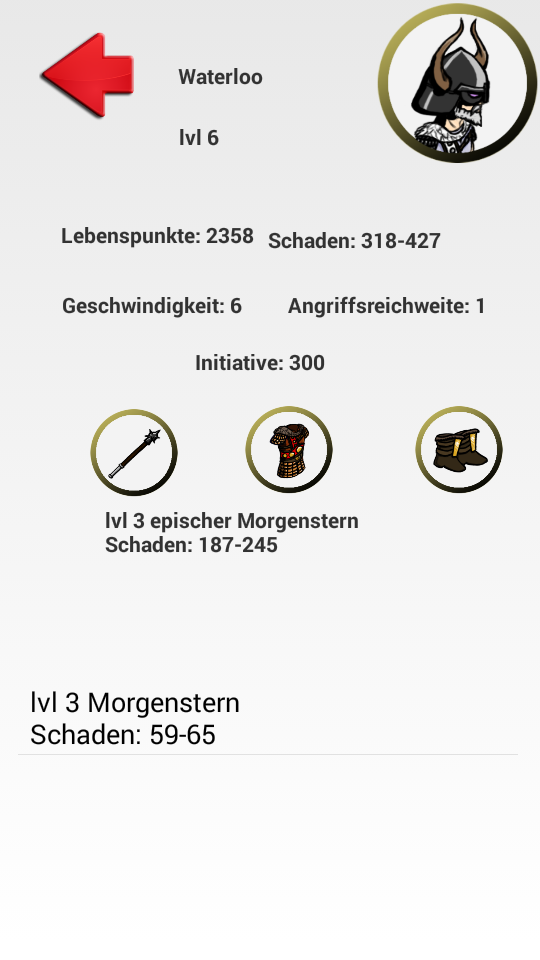
\includegraphics[width=0.6\textwidth]{statscreen.png}
	\caption{Ein Statusbildschirm}
\end{figure} 
Am Ende haben wir uns entschieden, vier unterschiedliche Klassen zu designen. Dies erlaubt es, die Klassen allein durch ihre Statuswerte zu spezialisieren. Eine Klasse kann viel Schaden überleben, eine auf lange Distanzen angreifen, eine macht viel Schaden und eine hat eine große Bewegungsreichweite. Dadurch wird ein Schere-Stein-Papier-Gameplay ermöglicht. So kann unser Fernkämpfer mehrere Schüsse auf die Klassen mit hohem Schaden und viel Leben abfeuern, bevor diese zurück angreifen können, während die Figur mit der großen Bewegungsreichweite gegen die Fernkampf-Klasse leichtes Spiel hat, aber den Kampf gegen die Klassen mit hohem Schaden und viel Leben verliert. Die Klasse mit viel Schaden ist kampfstärker als die Klasse mit viel Leben, während im Gegenzug die Klasse mit viel Leben mit gutem Spiel einen Großteil des Schadens einstecken kann und damit gegen die künstliche Intelligenz, die nach einem Muster bei der Wahl ihrer Ziele vorgeht, einen großen Vorteil erzeugen kann.
\\Die Spieler steuern im Kampf eine vorher ausgewählte Gruppe aus drei Figuren. Mehr Figuren hätten bedeutet, dass das Spielfeld größer sein müsste, um nicht überfüllt zu werden. Weniger hätte Tiefe aus der Gruppenerstellung und dem Kampf genommen. Aufgestellte Figuren bekommen Erfahrung und nach jedem Kampf wird ein Item aus einer zufälligen Itemgruppe und von zufälliger Stärke und Seltenheit (normal, selten, episch) fallengelassen. Wenn ein Spieler eine Waffe findet, hängt ihr Typ von den besiegten Figuren ab. Seltene Items sind um einen Faktor zwei beziehungsweise vier stärker, sodass ein episches Item massive Auswirkungen auf die Stärke einer Figur hat.
\\Wenn eine Figur genug Erfahrung sammelt, steigt ihr Level. Dies führt zu einer Steigerung ihrer Schadens- und Initativ-Werte sowie ihrer Lebenspunkte um 10-20\%, wobei der genaue Wert zufällig ist. Es wurde sich entschieden, die Steigerung von den momentanen Werten abzüglich der Items abhängig zu machen, sodass Charaktere ihre Statuswerte ungefähr alle fünf Level verdoppeln. Dies führt dazu, dass Fortschritt klar erkennbar ist, aber in einem absehbaren Rahmen bleibt.
\\Gegnergruppen setzen sich aus zufälligen Konstellationen der Klassen zusammen und bekommen zunehmend mehr Statuspunkte, um auszugleichen, dass sie keine Items tragen. Anfangs sind Gegner schwächer, weil Spieler noch keine Items haben. Damit Kämpfe abwechslungsreich sind, wird nicht nur drei gegen drei gekämpft, sondern es können auch einzelne oder auch zwei Gegner auftauchen. Damit die Kämpfe nicht trivial werden, haben zwei Gegner jeweils 25\% mehr Leben, Angriff und Initiative als gegnerische Figuren in Dreiergruppen, während ein einzelner Gegner, ein sogenannter Boss, eine Herausforderung darstellt. Er verfügt über 2,5-fache Statuswerte in Lebenspunkten, Schaden und Initiative, hat ein deutlich vergrößertes Modell, ist dadurch optisch gut erkennbar und gibt bessere Belohnungen. Damit Boss-Kämpfe außergewöhnlich bleiben, treten sie deutlich seltener auf. Das Gegner-Level hängt ungefähr vom Durchschnitts-Level der aktiven Spielerfiguren ab, wobei Gegnergruppen aus zwei Gegnern häufiger und Bosse immer ein höheres Level haben. Gegnergruppen werden auf der Karte abhängig von ihrem Level und ihrer Anzahl in Schwierigkeiten unterteilt, die an der Farbe ihres Informations-Fensters erkennbar ist.
\\Bei den Items wurde sich für drei unterschiedliche Typen entschieden. Waffen erhöhen den Schaden und tauchen in unterschiedlichen Formen auf, die jeweils nur von einer Klasse getragen werden können. Dies ermöglicht uns, Waffen für die Klassen einzeln anzupassen und zu verhindern, dass z.B. die Fernkampf-Klasse auf lange Distanzen nahezu den gleichen Schaden verursacht, wie die Klasse mit hohem Schaden. Rüstungen erhöhen die Lebenspunkte und kommen ebenso wie unsere dritte Kategorie, Schuhe, nur in einer Variante vor, die von allen Klassen tragbar ist. Schuhe erhöhen die Initiative und geben einen kleinen Bonus auf Lebenspunkte, während seltenere Formen zusätzlich die Bewegungsreichweite erhöhen.
\\Unsere Quests unterteilen wir in kleine und große Quests. Während kleine Quests in der Regel innerhalb einer Stunde abschließbar sein und für eher kurze Zeit fesseln sollen, sind große Quests dazu gedacht, Spielern über einen längeren Zeitraum ein Ziel zu geben. Dadurch wird für Langzeit-Motivation gesorgt.
\newpage
\section{Implementierung}
Die Implementierung umfasste mehrere verschiedene Teilaspekte und Sprachen sowie das Erstellen von Grafik und Menüs, wobei Martin Groppe die Android-App und das eigentliche Kampfmodul programmierte und Malte Kremer die Grafik, die Questtexte und die Erstellung des Siegesbildschirms in Unity übernommen hat. Game-Design und Menüführung wurden gemeinschaftlich erstellt, wobei Martin Groppe mehr Zeit beim Erstellen der Android Menüs investierte und Malte Kremer einen größeren Fokus auf das Gamedesign und die Konzeption gelegt hat.
\subsection{Karte und Menüs auf Android}
Unser Android-Code besteht aus vier Activities. Diese werden im folgenden nun einzeln beschrieben.
\begin{figure}[H] 
		\centering
		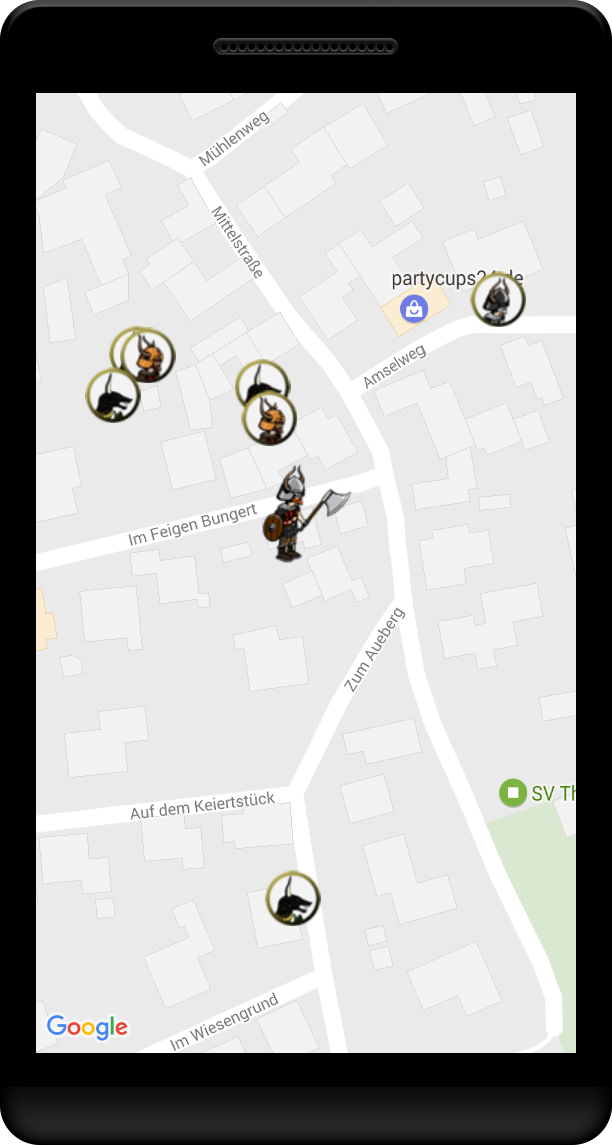
\includegraphics[width=0.6\textwidth]{map.png}
		\caption{Karte mit Spielfigur in der Mitte. Die Portraits in den Kreisen repräsentieren Gegnergruppen}
		\label{map}
\end{figure}
\subsubsection{Haupt-Activity und Karte}Die Haupt-Activity , auf der der Benutzer startet, besteht aus drei Fragmenten, zwischen denen man hin- und herwechseln kann, indem man mit dem Finger über den Bildschirm wischt. In der Mitte befindet sich die Karte der realen Umgebung (Abb.\ref{map}), in der sich der Spieler befindet. Auf ihr wird die Position des Spielers, die über Googles Location Service abgerufen wird, sowie die Position von Gegnergruppen, gegen die man kämpfen kann, angezeigt. Wird eine Gegnergruppe angeklickt, werden in einem Fenster Informationen zu den Gegnern angezeigt. Über dieses Fenster können Spieler den Kampf starten, wenn die Distanz zwischen ihnen und dem virtuellen Marker geringer als 20 Meter beträgt. Die notwendigen Daten für den Kampf werden als Json Strings serialisiert und der Activity, mit der Unity ausgeführt wird, über den Intent mitgeteilt. Json, kurz für Java Script Object Notation, ist ein kompaktes Datenformat, in dem man leicht Java Objekte serialisieren kann. Wir verwenden es auch um die Daten unserer Heldengruppe abzuspeichern.	
\newpage
\begin{figure}[H] 
		\centering
		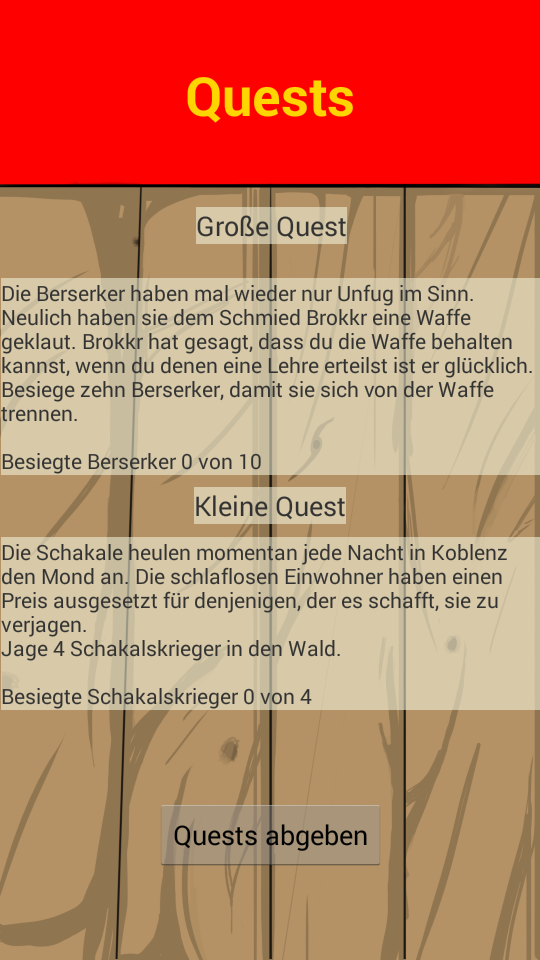
\includegraphics[width=0.6\textwidth]{questfragment.png}
		\caption{Questfragment mit momentan aktiven Aufgaben}
		\label{questfragment}
\end{figure}
\subsubsection{Quest-Fragment}
Im rechten Fragment der Haupt-Activity, das wiederum durch ein Wischen mit dem Finger über den Bildschirm erreicht wird, befindet sich eine Anzeige für momentane Aufgaben mit etwas erzählerischem Text\ref{questfragment}, die der Spieler erfüllen kann, um zusätzliche Belohnungen zu erhalten. Wenn der Spieler die jeweilige Aufgabe erfüllt hat, kann er diese über den Button abgeben und er bekommt einen zufälligen Gegenstand auf dem Level seiner Gruppe als Belohnung.
	
	
\newpage
\begin{figure}[H] 
		\centering
		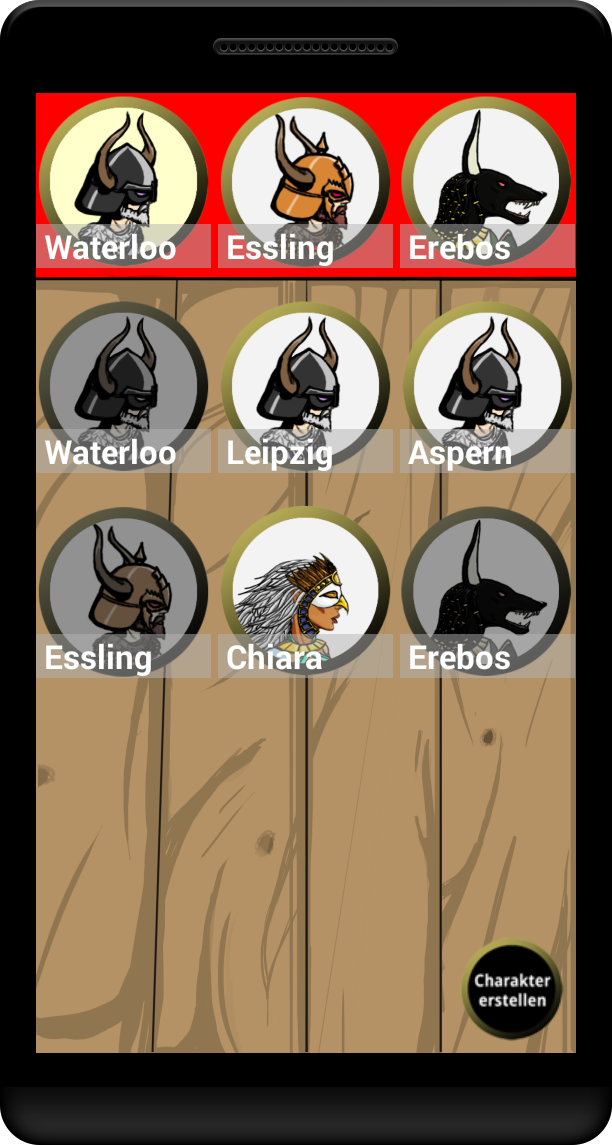
\includegraphics[width=0.6\textwidth]{charfragment.png}
		\caption{Charakter Fragment. Die aktive Party ist in der roten Leiste. Waterloo wurde angeklickt um ihn auszutauschen. Die möglichen Ziele für den Tausch sind Leipzig, Aspern und Chiara}
		\label{charfragment}
\end{figure} 
\subsubsection{Gruppen-Bildschirm}
Im linken Fragment befindet sich der Gruppen-Bildschirm (Abb.\ref{charfragment}). Auf ihm wird dem Spieler die eigene Gruppe angezeigt und er kann auswählen, welche Charaktere am Kampf teilnehmen sollen. Die Charaktere in der oberen roten Leiste sind momentan aktiv und man kann sie gegen einen beliebigen inaktiven Charakter austauschen, indem man sie und anschließend den Charakter, den man aktiv setzen will, anklickt.
Wenn man auf einen Charakter im unteren Teil klickt, wird die Activity zur Darstellung der Statuswerte gestartet und ihr werden mit einem Intent die Daten des angeklickten Charakters übergeben. Über den Button 'Charakter erstellen' unten rechts wird eine Activity gestartet, die dem Spieler ermöglicht, neue Charaktere zu erstellen.
\newpage
\begin{figure}[H] 
		\centering
		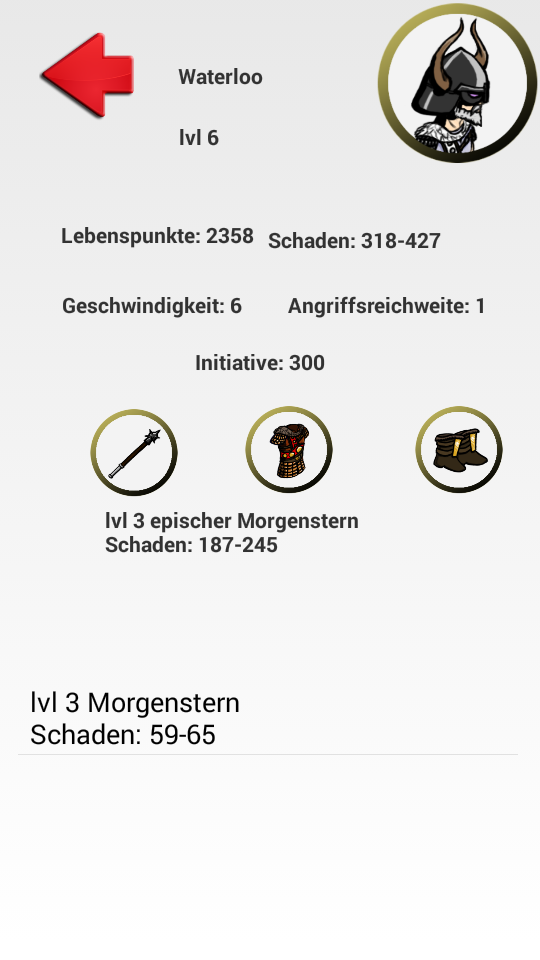
\includegraphics[width=0.6\textwidth]{statscreen.png}
		\caption{Statusbildschirm von Waterloo. Unten kann man die momentan ausgerüstete Waffe austauschen. Über die drei Symbole kann man zwischen Waffen, Rüstungen und Schuhen wechseln.}
		\label{statscreen}
\end{figure} 
\subsubsection{Statuswerte-Bildschirm}
Die Activity zur Darstellung der Statuswerte(Abb.\ref{statscreen}) zeigt alle Werte der Figur an, über die sie aufgerufen wird. Außerdem kann man hier die Figur mit gewonnenen Gegenstände ausrüsten, um ihre Statuswerte zu verbessern.
\newpage
\begin{figure}[H] 
		\centering
		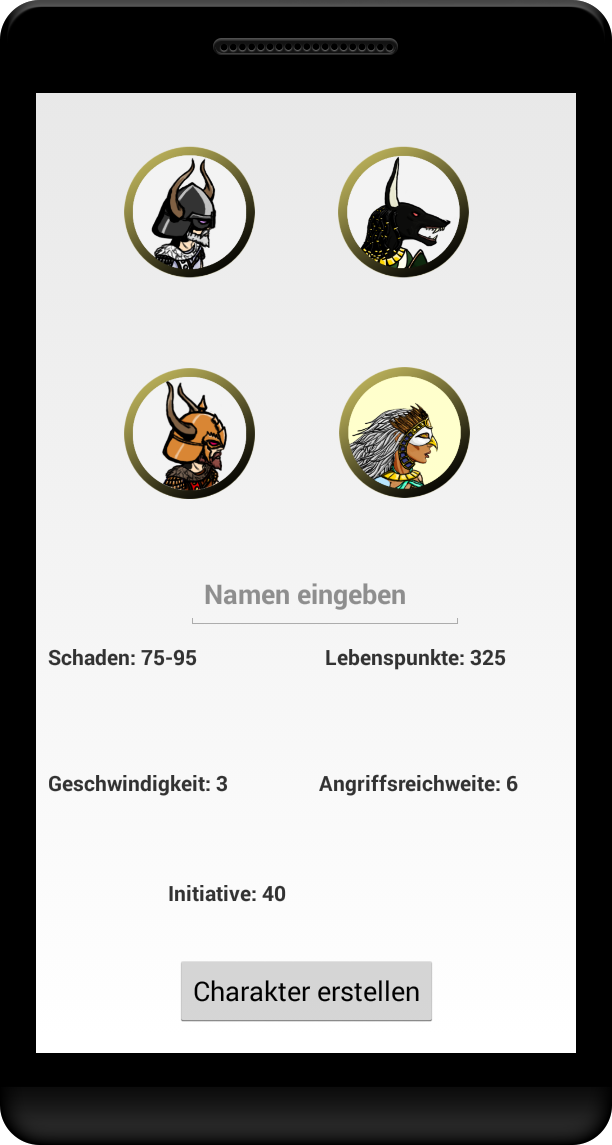
\includegraphics[width=0.6\textwidth]{createcharscreen.png}
		\caption{Hier kann man einen neuen Charakter erstellen.}
		\label{createcharscreen}
\end{figure} 
\subsubsection{Activity zum Erschaffen von Charakteren}
In der vierten Activity (Abb.\ref{createcharscreen}) kann man sich aus den vorhandenen Klassen weitere Figuren erstellen. Über die vier Bilder kann man die Klasse des Charakters aussuchen und über das Textfeld einen Namen eingeben. Die Activity zeigt einem zusätzlich die Basis-Statuswerte der momentan ausgewählten Klasse an. Diese unterscheiden sich klassen-abhängig stark.
\newpage
\begin{figure}[H]
		\centering
		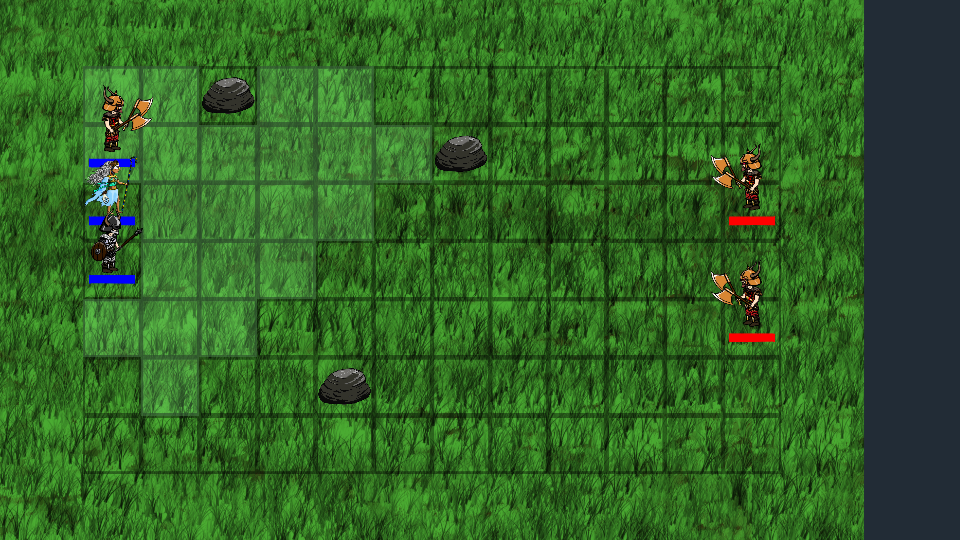
\includegraphics[width=1.0\textwidth]{fightscreen.png}
		\caption{Kampfactivity. Die Figuren mit blauem Lebenspunktbalken gehören dem Spieler. Die mit rotem sind die AI gesteuerten Gegner.}
		\label{fightscreen}
\end{figure}
\subsubsection{Unity/Kampf-Activity}
In der auf der Karte aufgerufenen Kampf-Activity (Abb.\ref{fightscreen}) kann der von Unity kompilierte Code abgespielt werden. Um zwischen Java und Unity-Code zu kommunizieren, verwenden wir Java Native Interface, kurz JNI. JNI ist eine Programmierschnittstelle, die es uns erlaubt, von Unity aus Java Funktionen aufzurufen, die sich in unserer Kampf-Activity befinden. Wir benutzen JNI, um die Kampfinformationen, die der Activity mitgeteilt werden, im Unity-Code aufzurufen und um zurück zur Haupt-Activity zu kommen, nachdem der Kampf abgeschlossen ist.
\newpage
\subsection{Erstellung des Kampfes in Unity}
In Unity werden Gameobjects als Basiseinheit für die Erstellung von Spielen verwendet. Gameobjects sind Behälter, denen man verschiedene Komponenten wie Sprites und Skripte hinzufügen kann. %<--- würde ich in Grundlagen packen
Für die Steuerung unseres rundenbasierten Kampfes generieren wir in Unity ein Gitter aus Quadraten, die sich anklicken lassen und ihre Position im Gitter kennen. Damit Kämpfe abwechslungsreicher sind, erzeugen wir zufällig auf unseren Quadraten Steine als Hindernisse, die Felder blockieren.\\ Anschließend werden aus unseren sogenannten Prefabs, Schablonen aus denen man ein Gameobject instanziieren kann, die am Kampf beteiligten Spielfiguren erzeugt und an die Ränder des Spielfeldes gesetzt. Figuren sind nun reihum am Zug. Wenn eine Figur, die dem Spieler gehört, an der Reihe ist, markieren wir alle Felder, zu denen sie sich bewegen kann mit einem hellgrünen Rand und einem helleren Untergrund. Dadurch kann der Spieler den Raum, innerhalb dessen sich die Figur bewegen kann, besser erkennen. Wird eines dieser Felder angeklickt, generieren wir wie in \ref{Pfadfindung} beschrieben einen Pfad, den unsere Figur dann entlangläuft. In unseren Prefabs sind die zugehörigen Animationen für die verschiedenen Befehle vorgemerkt. Wenn der Benutzer auf eine gegnerische Figur in Reichweite der aktiven eigenen Figur klickt, wird diese angegriffen und der Zug beendet. Alternativ kann man die eigene Figur anklicken, um den Zug ohne Angriff zu beenden. Wenn die aktive Figur dem Gegner gehört, übernimmt eine simple künstliche Intelligenz (fortan AI genannt) die Entscheidungen, die sonst der Spieler trifft. Die AI überprüft, ob eine feindliche Figur in Reichweite ist und greift diese, falls möglich, an. Wenn nicht, bewegt sie sich auf die nächste feindliche Figur auf dem Feld zu. Falls sie nun in Reichweite ist, greift sie die Figur an, andernfalls beendet sie ihren Zug.
\subsection{A*-Pfadfindung}\label{Pfadfindung}
Um Figuren auf unserem Spielfeld zu bewegen, benötigen wir einen Suchalgorithmus, um einen Pfad zu finden. Wir haben dazu den sogenannten A*-Algorithmus implementiert. Im Gegensatz zu uninformierten Suchalgorithmen wie z.B. Dijkstra wird in A* eine Heuristik benutzt, um zielgerichtet zu suchen. Alle Felder werden in drei Gruppen unterteilt. \\Die erste Gruppe sind die Felder, zu denen noch kein Weg gefunden wurde. Am Anfang sind dies alle außer dem Startfeld. \\Die zweite Gruppe sind die Felder, zu denen mindestens ein Weg bekannt ist. Diese werden, zusammen mit einem Wert f(x), in einer Liste gespeichert. Der Wert von f(x) ergibt sich aus der Summe der Kosten g(x), um das Feld zu erreichen, und den geschätzten Kosten h(x), um von dort zum Ziel zu kommen. Im Falle unseres Spiels kostet es einen Punkt, um sich orthogonal und zwei, um sich diagonal zu bewegen. Die Schätzfunktion ergibt sich aus der Summe der Abstände in x- und y-Koordinate zwischen einem Feld und dem Zielfeld. Zusätzlich wird für jedes Feld in dieser sogenannten Open List vermerkt, von welchem Feld ausgehend der momentane Weg dort ankommt. \\Die dritte Gruppe besteht aus den Feldern, zu denen bereits ein optimaler Weg gefunden wurde. Diese Felder werden in der sogenannten Closed List ebenfalls mit dem Feld, von dem der kürzeste Weg zu ihm ausgeht, gespeichert.
	
Zu Beginn befindet sich nur das Startfeld in der Open List und die Closed List ist leer. Nun wird in jedem Schritt das Feld a mit dem geringsten f-Wert aus der Open List in die Closed List aufgenommen. 
	
Für jedes Nachbarfeld b wird nun g(b) berechnet aus g(a)+1, falls es ein orthogonaler Nachbar, und g(a)+2, falls es ein diagonaler Nachbar ist. Zusammen mit der oben beschriebenen Heuristik wird nun f(b) = g(b)+h(b) berechnet und b wird in die Open List mit a als Vorgänger aufgenommen, falls es dort nicht schon mit einem gleichgroßen oder kleineren f-Wert vorhanden ist. Der Algorithmus endet, sobald das Zielfeld in die Closed List aufgenommen wird. Der Weg ergibt sich nun, indem man über die gemerkten Vorgänger die Felder bis zum Start zurückverfolgt. Zum besseren Verständnis folgt nun ein Beispiel für die Pfadfindung mit Bildern (Abb. \ref{pathfinding1} bis \ref{pathfinding5}).
\begin{figure}[H]
		\centering
		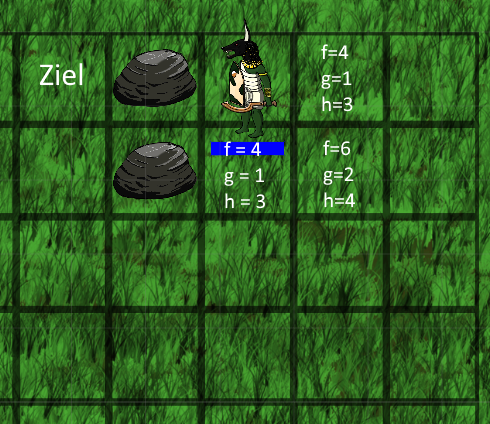
\includegraphics[width=0.8\textwidth]{pathfinding1.png}
		\caption{Der Schakalskrieger sucht einen Weg zum Ziel. Im ersten Schritt werden die Nachbarfelder mit ihrem f, g und h Werten in die Open List eingetragen.}
		\label{pathfinding1}
\end{figure}
\begin{figure}[H]
		\centering
		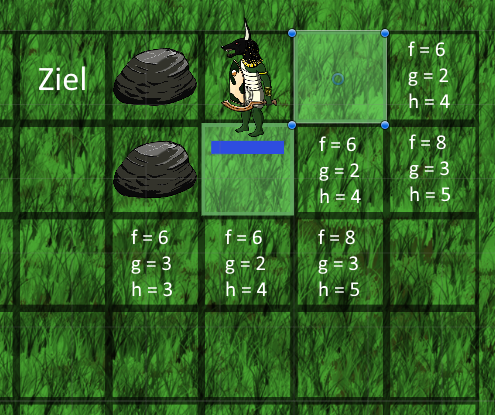
\includegraphics[width=0.8\textwidth]{pathfinding2.png}
		\caption{Die Felder mit f = 4 wurden nun in die Closed List übernommen (markierte Felder). Für ihre Nachbarn wurde der f Wert berechnet und sie wurden in die Open List aufgenommen}
		\label{pathfinding2}
\end{figure}
\begin{figure}[H]
		\centering
		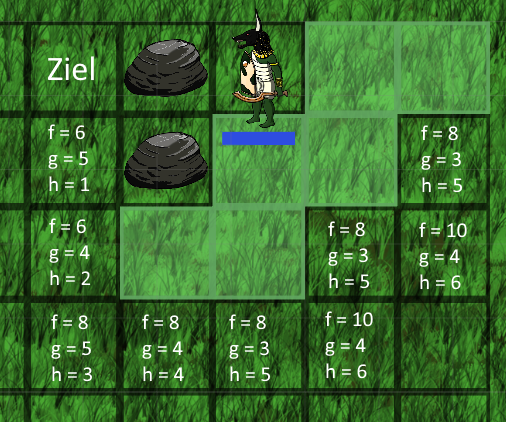
\includegraphics[width=0.8\textwidth]{pathfinding3.png}
		\caption{Die kleinsten f-Werte aus der Open List wurden wieder in die Closed List aufgenommen.}
		\label{pathfinding3}
\end{figure}
\begin{figure}[H]
		\centering
		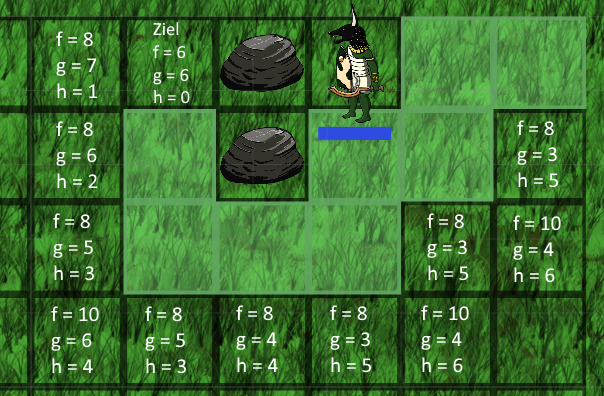
\includegraphics[width=0.9\textwidth]{pathfinding4.png}
		\caption{Das Zielfeld ist jetzt in der Open List angekommen. Da es den kleinsten f-Wert hat, sind wir im nächsten Schritt fertig.}
		\label{pathfinding4}
\end{figure}
\begin{figure}[H]
		\centering
		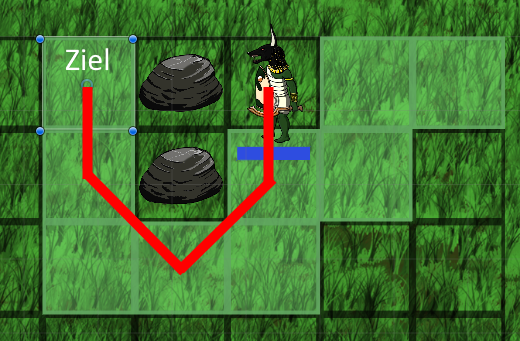
\includegraphics[width=0.8\textwidth]{pathfinding5.png}
		\caption{Das Ziel ist nun in der Closed List. Der Pfad ergibt sich nun dadurch, dass sich jedes Feld gemerkt hat, von welchem Vorgänger aus der kürzeste Weg zu ihm führt.}
		\label{pathfinding5}
\end{figure}
\newpage
\subsection{Der Sieg-Bildschirm}
Nachdem eine Seite keine Figuren mehr hat, endet der Kampf. Hat der Spieler verloren, ruft die Unity-Activity wieder die Karte auf und wird beendet. Hat der Spieler gewonnen, wird ihm das mitgeteilt und er bekommt Erfahrung und ein Item als Belohnung. Zur Darstellung dessen wird in Unity eine neue Scene aufgerufen und die alte verworfen. Der Siegesbildschirm liest aus dem Json-Objekt die notwendigen Daten aus und stellt den Erfahrungsfortschritt mit Balken dar, die neben den Namen und Gesichtern der Figuren angezeigt werden. 
\begin{figure}[H]
		\centering
		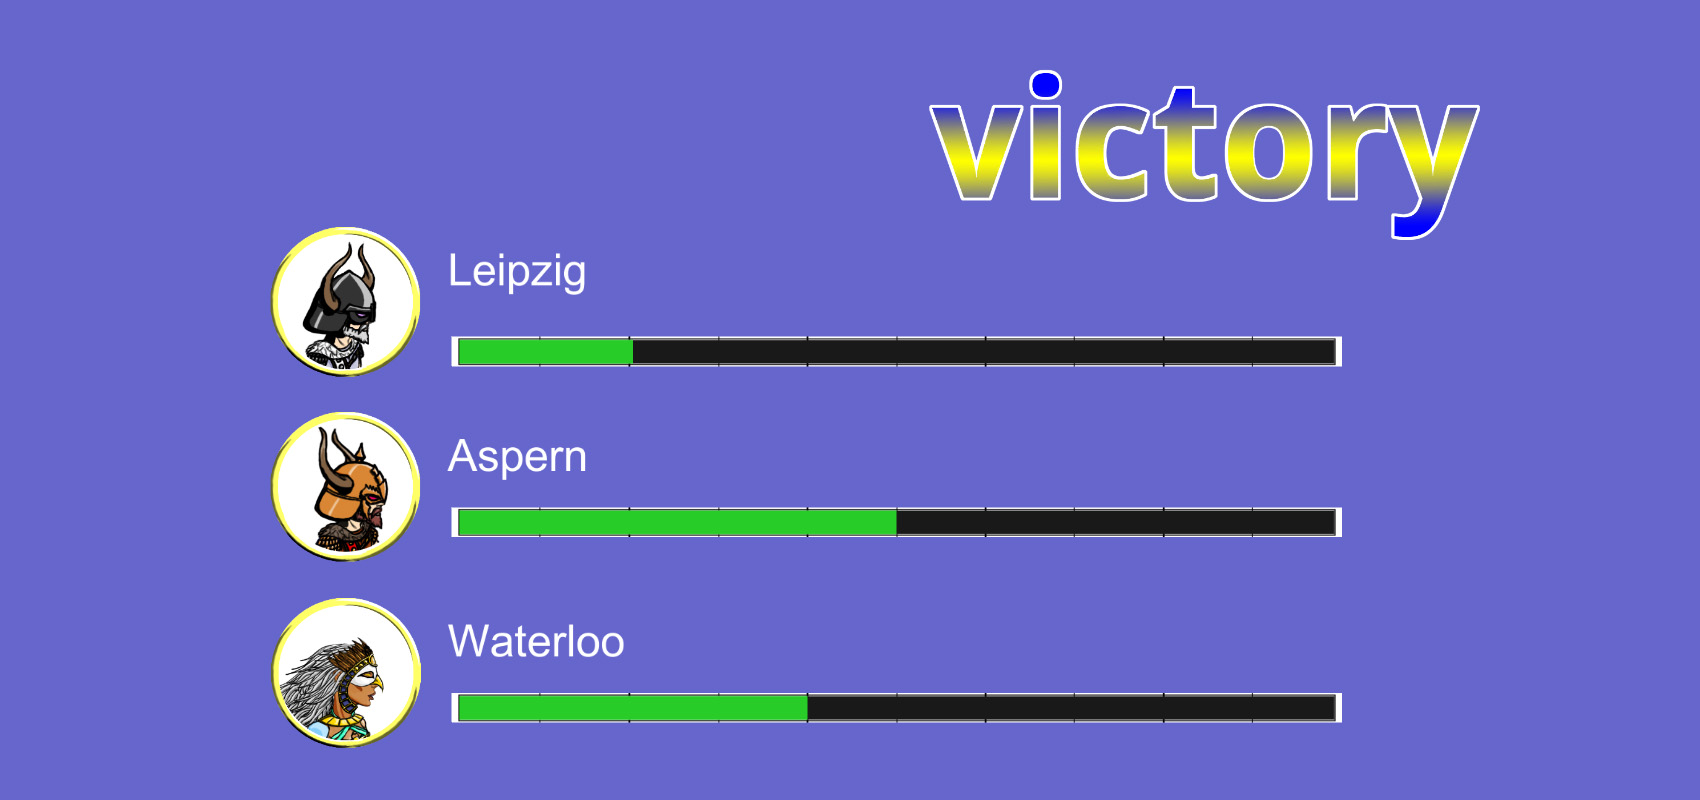
\includegraphics[width=1\textwidth]{sieg1}
		\caption{die erste Anzeige des Sieg-Bildschirm}
\end{figure}
Danach löscht Unity die Erfahrungsbalken, Namen und Gesichter und stellt das ebenfalls aus dem Json-Objekt ausgelesene Item dar. Nach sechs Sekunden wird die Unity-Activity beendet und die Karte wieder aufgerufen.
\begin{figure}[H]
		\centering
		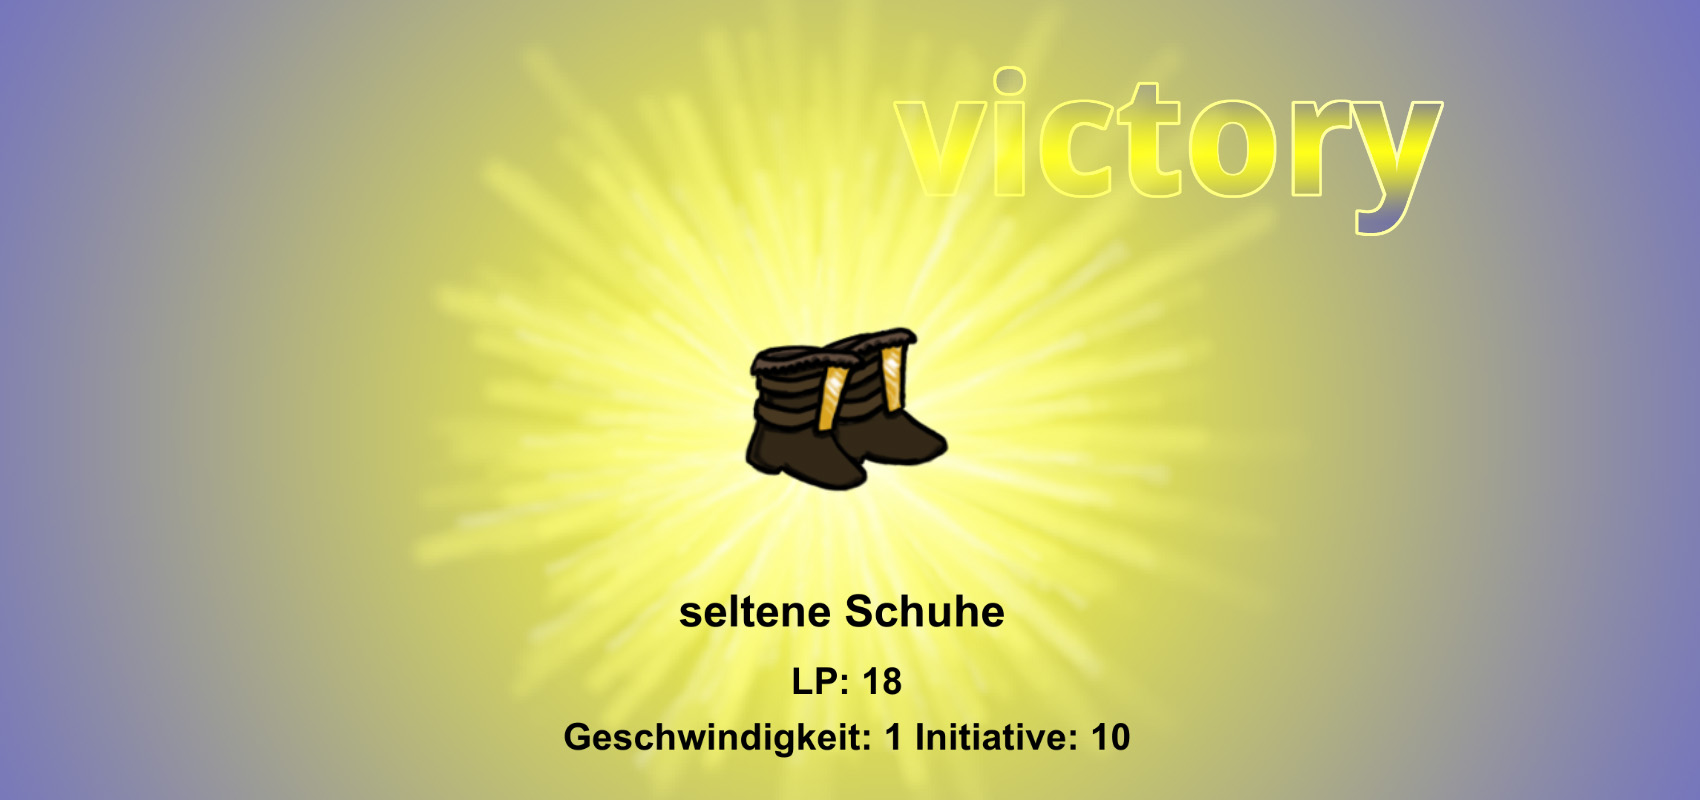
\includegraphics[width=1\textwidth]{sieg2}
		\caption{die Präsentation des Items}
\end{figure}
\newpage
\subsection{Grafik und Stil}
Der Stil hatte den Anspruch, sowohl auf Smartphones als auch auf Tablets gut auszusehen, ein breites Publikum anzusprechen und sich vom Gewöhnlichen abheben. Das hieß, dass es mehrere Herausforderungen zu meistern gab:
\begin{enumerate}
	\item 
 Die größten Tablet-Bildschirme wie die des Google Pixel C können eine Bildschirmdiagonale von mehr als 25cm haben, während unser Test-Smartphone z.B. gerade mal 11cm hat. Unser Spiel sollte auf beiden Bildschirmen gut aussehen und erkennbar sein. Realistischere Darstellungen (siehe Abb. \ref{speerträger}) waren auf dem Test-Smartphone kaum erkennbar (siehe Abb. \ref{speerkarte}), sodass wir uns für einen Comic-Look mit unrealistischen Proportionen entschieden haben. Dabei galt es, eine gute Balance zu finden zwischen stark unterschiedlichen Proportionen der Figuren, was insbesondere ältere Spieler häufig abschreckt, und Erkennbarkeit auf kleinen Bildschirmen durch auffällige vergrößerte Merkmale.
\begin{figure}[H]
		\centering
		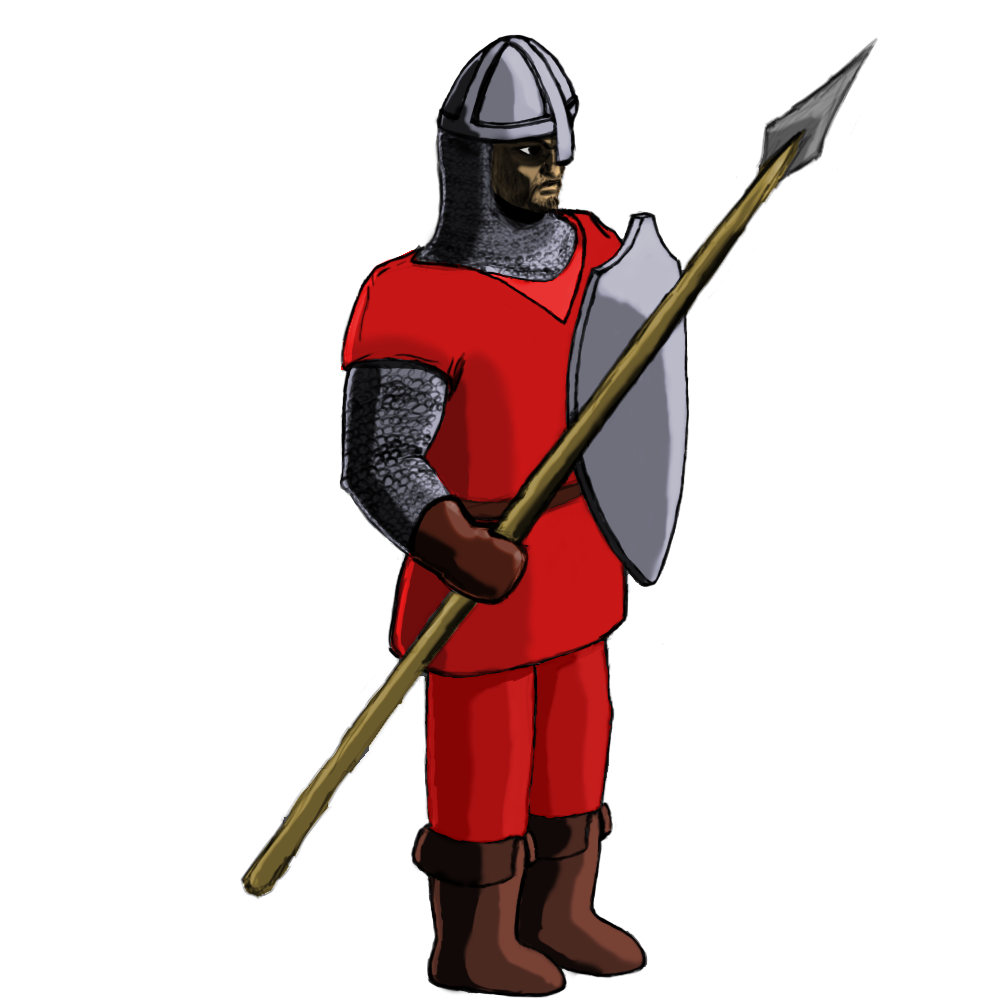
\includegraphics[height=5cm]{soldier.png}
		\caption{Früher Entwurf eines Speerträgers}
		\label{speerträger}
\end{figure}
\begin{figure}[H]
		\centering
		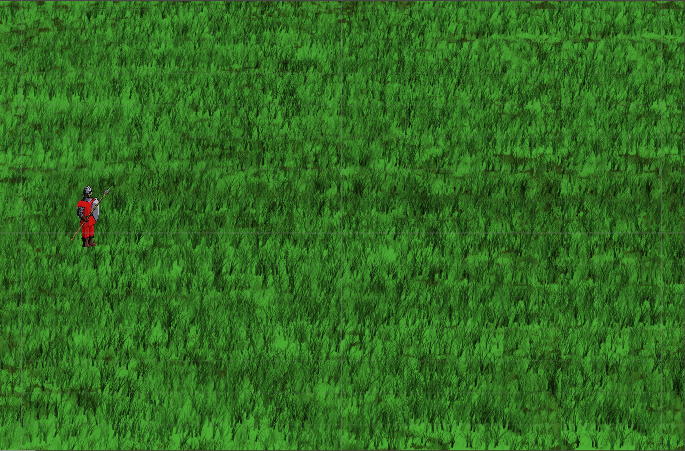
\includegraphics[width=13cm]{soldierbackground.png}
		\caption{Speerträger auf unserem Schlachtfeld}
		\label{speerkarte}
\end{figure}
\item Das Spiel sollte Erwachsene und Jugendliche anziehen und fesseln, aber immer noch bedenkenlos von Kindern spielbar sein. Das bedeutete für die Umsetzung unserer Grafik, dass der Grafikstil nicht zu düster sein durfte, aber auch nicht zu kindlich, ohne austauschbar zu wirken.
\item Die hohe Detaildichte, welche für die Entwicklung für Tablets erforderlich ist, benötigt einen großen Zeitaufwand. Folglich mussten Animationen vom Grundmodell aus einfach zu erzeugen sein und eine Ansicht gewählt werden, in der dies sich nicht negativ auf die Optik des Spiels auswirkt.
\end{enumerate}
Die meisten Taktik-Rollenspiele haben sehr abwechslungsreiche und tendenziell zufällige Karten mit teils zufälligen Startpositionen und verschiedenen Terrain-Höhen. Da allerdings unser Fokus stärker auf strategischen als zufälligen Kämpfen lag, entschieden wir uns bei dem Aufbau des Schlachtfeldes für ein flaches Feld mit Gegnern auf der einen und Spielern auf der anderen Seite, wie es in Strategie-Spielen wie Schach oder der Heroes-Serie zum Einsatz kommt. Dies erleichterte auch das Grafikdesign, da Figuren sich hauptsächlich auf der horizontalen Achse bewegen, sodass eine 3/4-Ansicht mit situationaler Spiegelung für fast alle möglichen Lauf-Richtungen gut aussieht. Zusätzlich legten wir fest, das Feld breiter als hoch zu gestalten, was auf das Gameplay positive Auswirkungen hatte, und zudem bedeutete, dass zum einen das Schlachtfeld der 16:9-Auflösung der meisten Smartphones besser entspricht, zum anderen die optisch schlechter aussehenden Bewegungen nach gerade oben oder gerade unten seltener sind.
\\Danach wurden mehrere Skizzen erstellt, um eine geeignete Balance zwischen realistischem Look und übertriebem Comic-Look zu finden. So entschieden wir uns, den Kopf beziehungsweise Helm der Figuren zu vergrößern und als durchgängiges Identifikationsmerkmal zu verwenden. Erste Versuche (s. Abb. \ref{earlydesign}) waren stärker überzeichnet und an den sogenannte Chibi-Zeichenstil angelehnt, da ein vergrößerter Kopf leicht auszumachen ist und eine gute Differenzierung der verschiedenen Figuren ermöglichte. Es gab allerdings Bedenken, dass diese Optik Hardcore-Spieler abschrecken könnte, die wir ebenfalls ansprechen wollten. Daher wurde der Kopf in folgenden Versuchen etwas weniger überzeichnet, der restliche Körper etwas realistischer proportioniert. Zudem wurde die Bewaffnung ebenfalls etwas vergrößert. 
\\Da geplant war, einige Modelle durch farbliche Veränderung sowie das Abändern einiger Details als neue Modelle zu benutzen, erlaubte eine größere Waffe eine gute Erkennbarkeit von Elementen, die für Statuswerte wichtig sein sollten. So sollte der Spieler intuitiv verstehen können, dass die Figur mit dem Schild mehr Schaden aushält und die Figur mit den zwei Äxten mehr Schaden anrichtet. Dies wäre bei reinem Verändern der farblichen Gestaltung nicht möglich gewesen.

\begin{figure}[H]
		%	\raggedleft
		\centering
		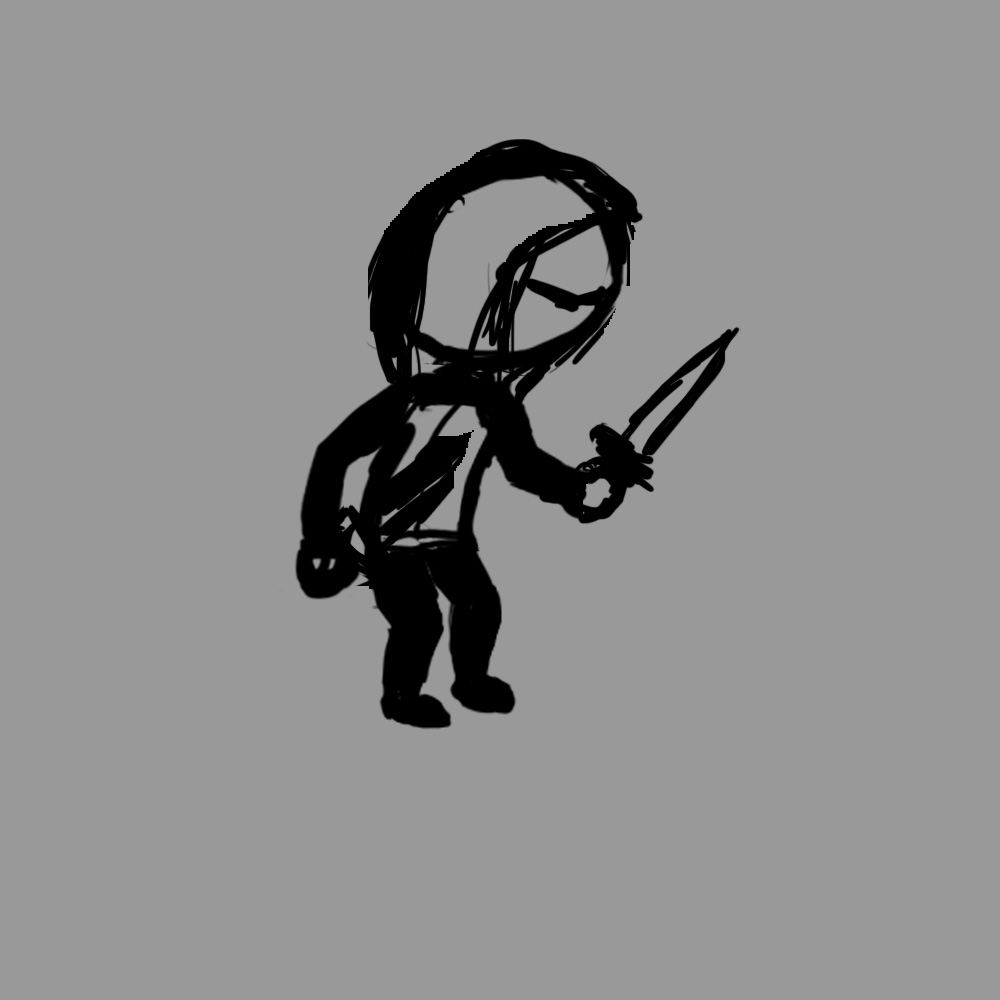
\includegraphics[width=.5\textwidth]{assachibi.jpg}
\end{figure}
\begin{figure}[H]
		\centering
		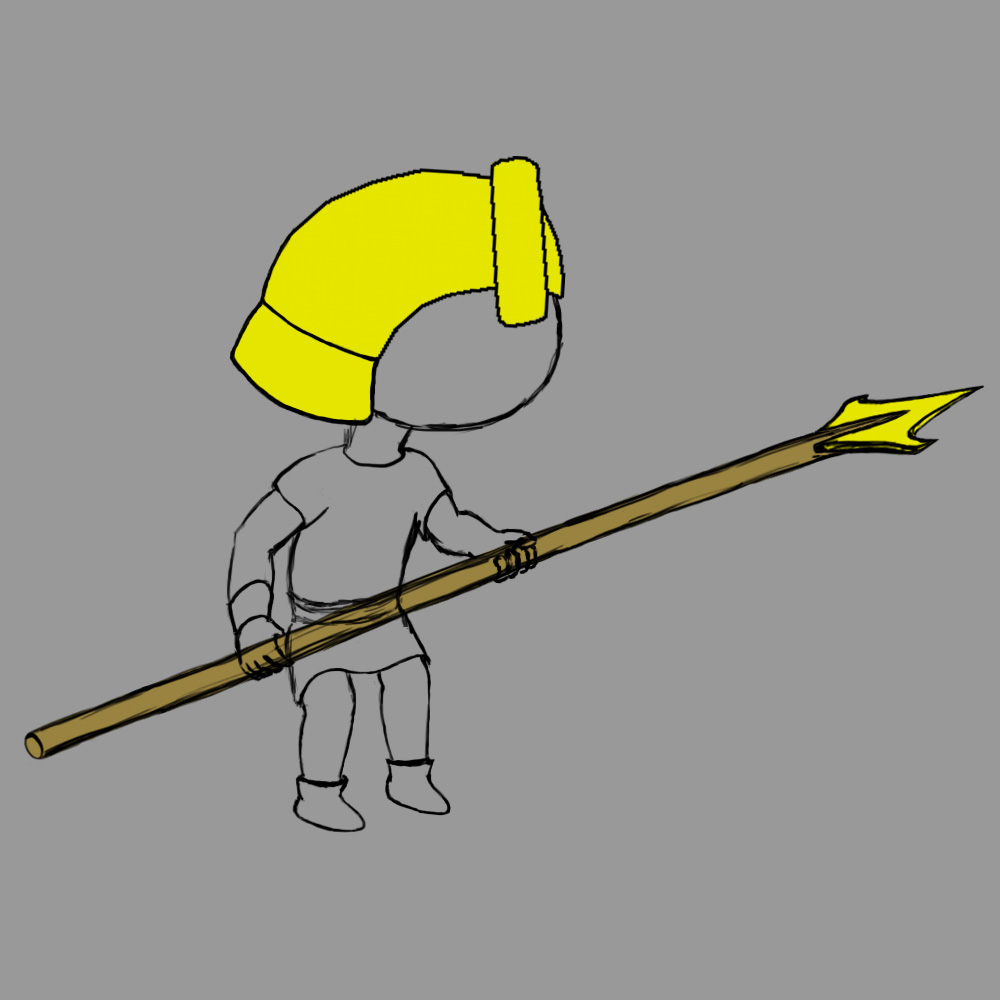
\includegraphics[width=.5\textwidth]{egychibi.jpg}
		\caption{Frühe Skizzen im Chibi-Stil}
		\label{earlydesign}
\end{figure}
\newpage
\subsection{Die Figuren}
\begin{figure}[H]
		\centering
		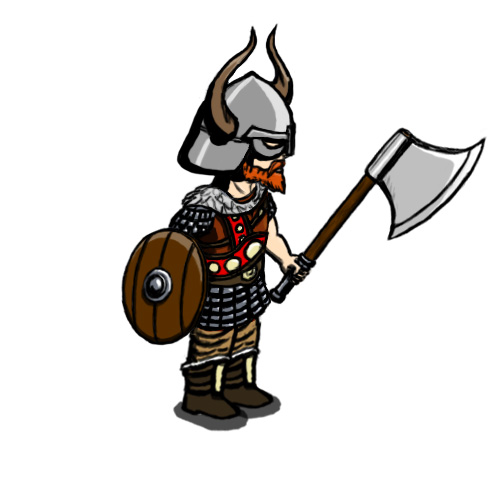
\includegraphics[height=8cm]{viking.jpg}
		\caption{Der finale Wikinger}
		\label{viking}
\end{figure}
\subsubsection{Der erste Wikinger}
Da die klassischen Fantasy-Skizzen zu kindlich oder zu generisch gerieten, wurden als zunehmend Motive abseits des Mainstreams verwendet. So wurde sich für ein Wikinger-Motiv entschieden, was es erlaubte, eine Figur düster und trotzdem niedlich aussehen zu lassen. Außerdem sind die gehörnten Helme in Medien ikonisch (wenn auch historisch falsch), sodass Spieler auch auf sehr kleinen Bildschirmen erkennen sollten, dass es sich um einen Wikinger handelt.
\\Wikinger sind seit dem 18. Jahrhundert als noble Wilde verklärt, sie werden aber seit dem frühen 20. Jh. auch häufig als heidnische, brutale Piraten\footnote{\url{https://en.wikipedia.org/wiki/Vikings}} dargestellt.%wikipedia
Attribute, die ihnen häufig zugeschrieben werden sind Wildheit, Unabhängigkeit, Kraft und Aggressivität. Darstellungen zeigen sie meistens als Krieger oder Seefahrer, oft mit Äxten und bemalten Holzschilden. Ihre Kleidung setzt sich in modernen Darstellungen aus mehreren Lagen von Kleidungsstücken oder Pelzen über leichten Rüstungen wie Kettenhemden zusammen (was historisch akkurat ist), dazu die ikonischen gehörnten Helme (die historisch falsch sind). In fantastischeren Darstellungen tragen sie oft mehrere Gürtel und Medallions und gelegentlich Lamellenpanzer (Metallplättchen, die auf Leder aufgenäht werden). Wikinger haben in modernen Darstellungen nahezu immer lange Haare und Bärte, beides häufig zu Zöpfen geflochten. 
\\Dementsprechend setzten wir den ersten Wikinger (s. Abb. \ref{viking}), der es in das finale Spiel schaffte, aus mehreren dieser Elemente zusammen. Er trägt einen auffälligen gehörnten Helm, eine Axt und ein hölzernes Rundschild. Die Axt und der Kopf/Helm sind bewusst vergrößert, um auch auf einem Handy-Bildschirm klar sichtbar zu sein. Die Rüstung setzt sich aus mehreren Gürteln mit Metallplättchen über einem roten Wams zusammen und wird durch Lamellenpanzer über Schulter und Waffenrock komplementiert. Die Detaildichte der Rüstung stört nicht auf dem Smartphone, da Axt, Schild und Helm den Wikinger klar erkennbar machen, durch sie sieht der Wikinger aber auf Tablets besser aus. Durch die Gürtel und Medallions setzt sich die Rüstung klar von 'normaler' mittelalterlicher Kleidung und Rüstung ab und der Lamellenpanzer lässt ihn kriegerisch aussehen. Zusätzlich trägt er einen Pelz um die Schultern und Pelzbesatz auf den Stiefelrändern sowie eine aus Pelz gemachte Hose, damit er einen 'wilden' Eindruck hinterlässt. Die Stiefel haben im Stile von Beinschienen einen metallenen Clip, um interessanter auszusehen. Dabei wurden Ränder der Figur bewusst schwarz, Lichtreflexionen z.B auf Helm und Axt plakativ und die Schatten mit geringen Farbverlauf gelassen, um die Figur vom Hintergrund abzuheben und einen Comic-Eindruck zu erzielen. Später ist die Figur unser Avatar Essling auf der Karte geworden.
	
\newpage
\subsubsection{Der Morgenstern-Wikinger}
\begin{figure}[H]
	\centering
	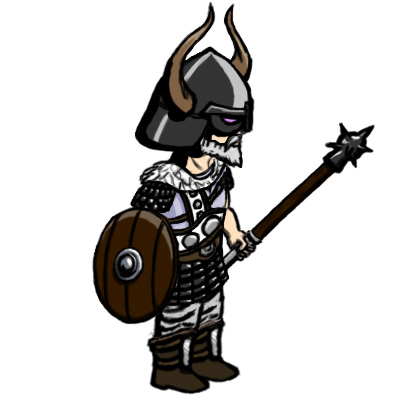
\includegraphics[height=8cm]{morningstar.jpg}
	\caption{Die kühle Kolorierung mit dem Morgenstern}
	\label{morningstar}
\end{figure}
Im Rahmen der Kolorierung des ersten Wikingers wurde sich stärker mit Farblehre auseinandergesetzt. So entstanden danach zwei 'Umfärbungen', eine Figur mit warmen und eine mit kalten Farben, mit dem Ziel, sie optisch stärker voneinander abzusetzen. Die Version mit den kühlen Farben wurde mit einem Morgenstern ausgestattet. Morgensterne sind stumpfe spezialisierte Waffen des Spätmittelalters, die dazu gedacht sind, schwere Rüstungen zu brechen. Sie sind also gleichzeitig eine Waffe, die rohe Kraft umsetzt, aber auch spezialisiert, also bedachter ist. Dies gibt ihm einen kalkulierenden Eindruck. Dies wird verstärkt durch den weißen Bart und die generell kühlen Farben, da kühle Farben häufig mit Rationalität in Verbindung gebracht werden.
\newpage
\begin{figure}[H]
	\centering
	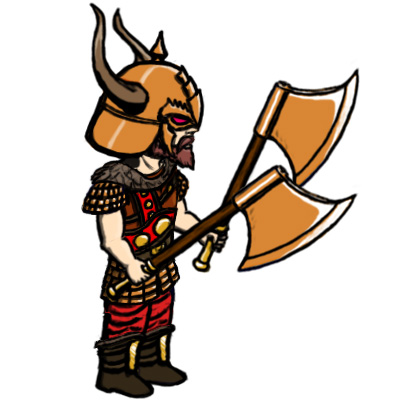
\includegraphics[height=5.5cm]{berserker.jpg}
	\caption{Der Berserker}
	\label{berserker} 
\end{figure}
\subsubsection{Der Berserker}
Die bekannteste mit Wikingern assoziierte Figur ist der Berserker, ein Krieger, der sich in einen Kampfrausch versetzte. Dieser kommt in vielen Spielen vor, nicht nur in Fantasy-Wikinger-Varianten wie den Chaos-Berserkern des populären Tabletops Warhammer, auf dem einige Spiele basieren, sondern auch in eher historisch angehauchten Titeln wie dem bekannten Strategie-Spiel Age of Empires 2 und in mehreren Teilen der hochgelobten  Civilization-Reihe. Berserker werden häufig als blutrünstig und wahnsinnig dargestellt. Dementsprechend wurde die warme Kolorierung der Berserker mit vielen rot-und orange-Tönen gestaltet, da rot häufig mit Aggression in Verbindung gebracht wird. Die Figur bekam zwei Äxte, um aggressiver zu wirken. Der bronze-farbige Helm wurde nach einem Drachenkopf modelliert, um die Assoziation mit rotem Feuer zu erzeugen und ihn stärker von den anderen beiden Wikingern abzuheben. Zuletzt entschieden wir uns, den finalen Wikinger (Abb.\ref{viking}) nicht in die Kämpfe aufzunehmen, da er einen Mittelweg zwischen dem ersten Berserker und dem Morgenstern-Wikinger darstellte und die Gefahr bestand, dass es zu Verwechslungen kommt.
\newpage
\begin{figure}[H]
	\centering
	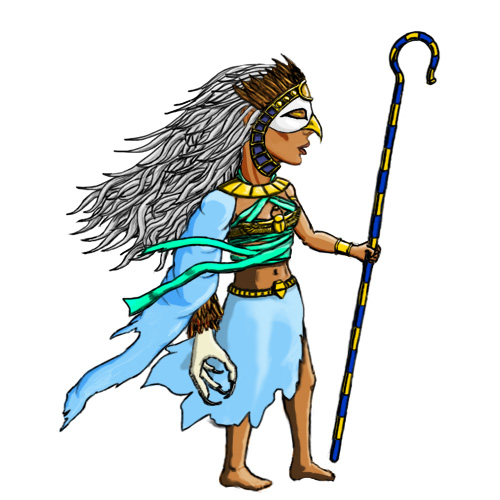
\includegraphics[height=6cm]{priestess.jpg}
	\caption{Die Priesterin des Ra}
	\label{priestess}
\end{figure}
\subsubsection{Die Priesterin des Ra}
Nachdem die Entscheidung für zwei Varianten von Wikingern gefallen war, suchten wir einen starken Kontrast, um das Spiel optisch interessant und abwechslungsreich zu halten. Mit dem ägyptischen Motiv, mit dem wir schon gedanklich und in der Entwurfsphase gespielt hatten, war ein geeignetes Motiv gefunden. Es eignete sich hervorragend, da es eher selten in Spielen Verwendung findet und einen starken optischen und kulturellen Kontrast zu den Wikingern bietet. Während Wikinger aufgrund ihrer militärischen Expansion und Piraterie im Mittelalter assoziativ mit roher Kraft, Kampfeslust und Barbarei verbunden werden und Unabhängigkeit sowie die Seefahrt in der Kultur eine große Rolle spielten, waren die Ägypter eine spirituell geprägte, künstlerische Hochkultur, die über Jahrtausende wenig expandierte und stark hierarchisch aufgebaut war. Außerdem sind die optischen Unterschiede stark, bedingt u. a. durch die unterschiedlichen Klima-Bedingungen und den historischen Zeitabstand. 
\\Die Entwicklung der Priesterin des Ra war aus mehreren Gründen ungewöhnlich komplex.
Nach den Wikingern gab es eine Reihe Vorgaben, die in den nächsten zwei Figuren erfüllt werden sollten. So war geplant, dass für die ägyptischen Figuren der mystische Aspekt ihrer Kultur im Vordergrund steht und sie aufgrund ihrer kulturellen Unterschiede spezialisierter sein beziehungsweise weniger auf rohe Kraft (und unsere Gameplay-Pendants Lebenspunkte und Schaden) setzen als die Wikinger. Die Idee formte sich, einen mobileren Nahkämpfer und einen Fernkämpfer, der möglicherweise göttliche Kräfte nutzte, zu entwerfen. Außerdem sollten die Figuren um eine weibliche Figur erweitert werden, sowohl um weiblichen Spielern eine Identifikationsfigur zu geben, als auch aus Gründen optischer Abwechslung. Zu Beginn der Konzeption dieser Figur bestand u. a. die Idee, einen männlichen Falken-Krieger als Nahkämpfer und die zweite ägyptische Figur zu einem weiblichen Fernkämpfer machen. Da die Waffe bereits vergrößert war, bot sich an, eine andersartige, auffällige Waffe zu konzipieren. Da die Bewaffnung der Wikinger eher realistisch gehalten wurde (abgesehen von der Größe), sollte die Waffe allerdings nicht zu fantastisch sein. So wurden verschiedene Konzepte skizziert, zunehmend als eine am Arm befestigte Waffe nach dem Vorbild einer Klaue oder eines Schnabels, bis die Entscheidung getroffen wurde, den Arm selbst zu einer Vogelklaue zu machen. Die Ägypter stellten ihre Götter mit Tierköpfen dar, was immer wieder Vorbild für moderne Webkunst ist. Ein anderes Körperteil abzuwandeln war also naheliegend. Da die Figur damit angreifen können sollte und mit Flügeln und Klauen den Harpyien (ein griechisches Fabelwesen mit Vogelkörper und Frauenkopf, häufig mit weiblichem Oberkörper abgesehen von den Flügeln) zu ähnlich wäre, wurde entschieden, einen Arm durch eine Klaue zu ersetzen.
\\Danach wurde die Entscheidung getroffen, die Figur weiblich zu machen. Bei Entwürfen zeigte sich, dass eine zierlichere Figur einen stärkeren Kontrast zu der monströsen Vogelklaue darstellen würde und der Figur erlaubte, sowohl tragisch als auch monströs zu wirken. Dies machte es leichter, sie auf der Seite des Spielers, aber auch auf Seite des Gegners zu erklären. Das bedeutete, dass die Proportionierung mehrfach angepasst wurde, denn die Figur musste insgesamt schmaler gestaltet werden. Dennoch sollte die Figur weiterhin gut erkennbar sein, d.h. Kopf und Arm müssten entsprechend der Waffen und Köpfe der Wikinger weiterhin groß und prägnant sein, ohne zu verzerrt zu wirken. 
\\Das ägyptische Motiv bedeutete mehr komplexe Materialien, die zu zeichnen waren, insbesondere Muskulatur, Masken, beweglicher Stoff, einen Priesterstab und Goldschmuck. Die populärsten ägyptischen Vogelgötter sind Horus, der Gott des Himmels und Ra, Gott der Sonne. Wir entschieden uns für Ra, da dessen Symbolik weiter verbreitet ist und angedacht war, die Figur zur Fernkämpferin zu machen und Feuerbälle für eine Fernkämpferin ein geeignetes Geschoss darstellten.
\\Die Priesterin bekam neben dem Arm eine Vogelmaske, ein Konzept, das noch aus der Zeit des Falken-Kriegers existierte und eine einfache Möglichkeit darstellte, das Gesicht interessanter und geheimnisvoller zu machen. Die Maske wurde mit zusätzlichen Federn versehen, um den Vogel-Eindruck noch zu verstärken. Außerdem bekam sie Bänder aus lila farbigen Edelsteinen mit aufgesetztem Gold nach dem losen Vorbild der Todesmaske des Tutanchamun, die einem von Pharaonen getragenen Kopftuch (Nemes) nachempfunden ist. Auf der Stirn wurde eine große rotgoldene Platte als Symbol für die Sonne gezeichnet, eine Abwandlung der historischen Darstellungen von Ra, der oft mit einer gewaltigen roten Scheibe über seinem Kopf abgebildet ist.
\begin{figure}[H]
	\centering
	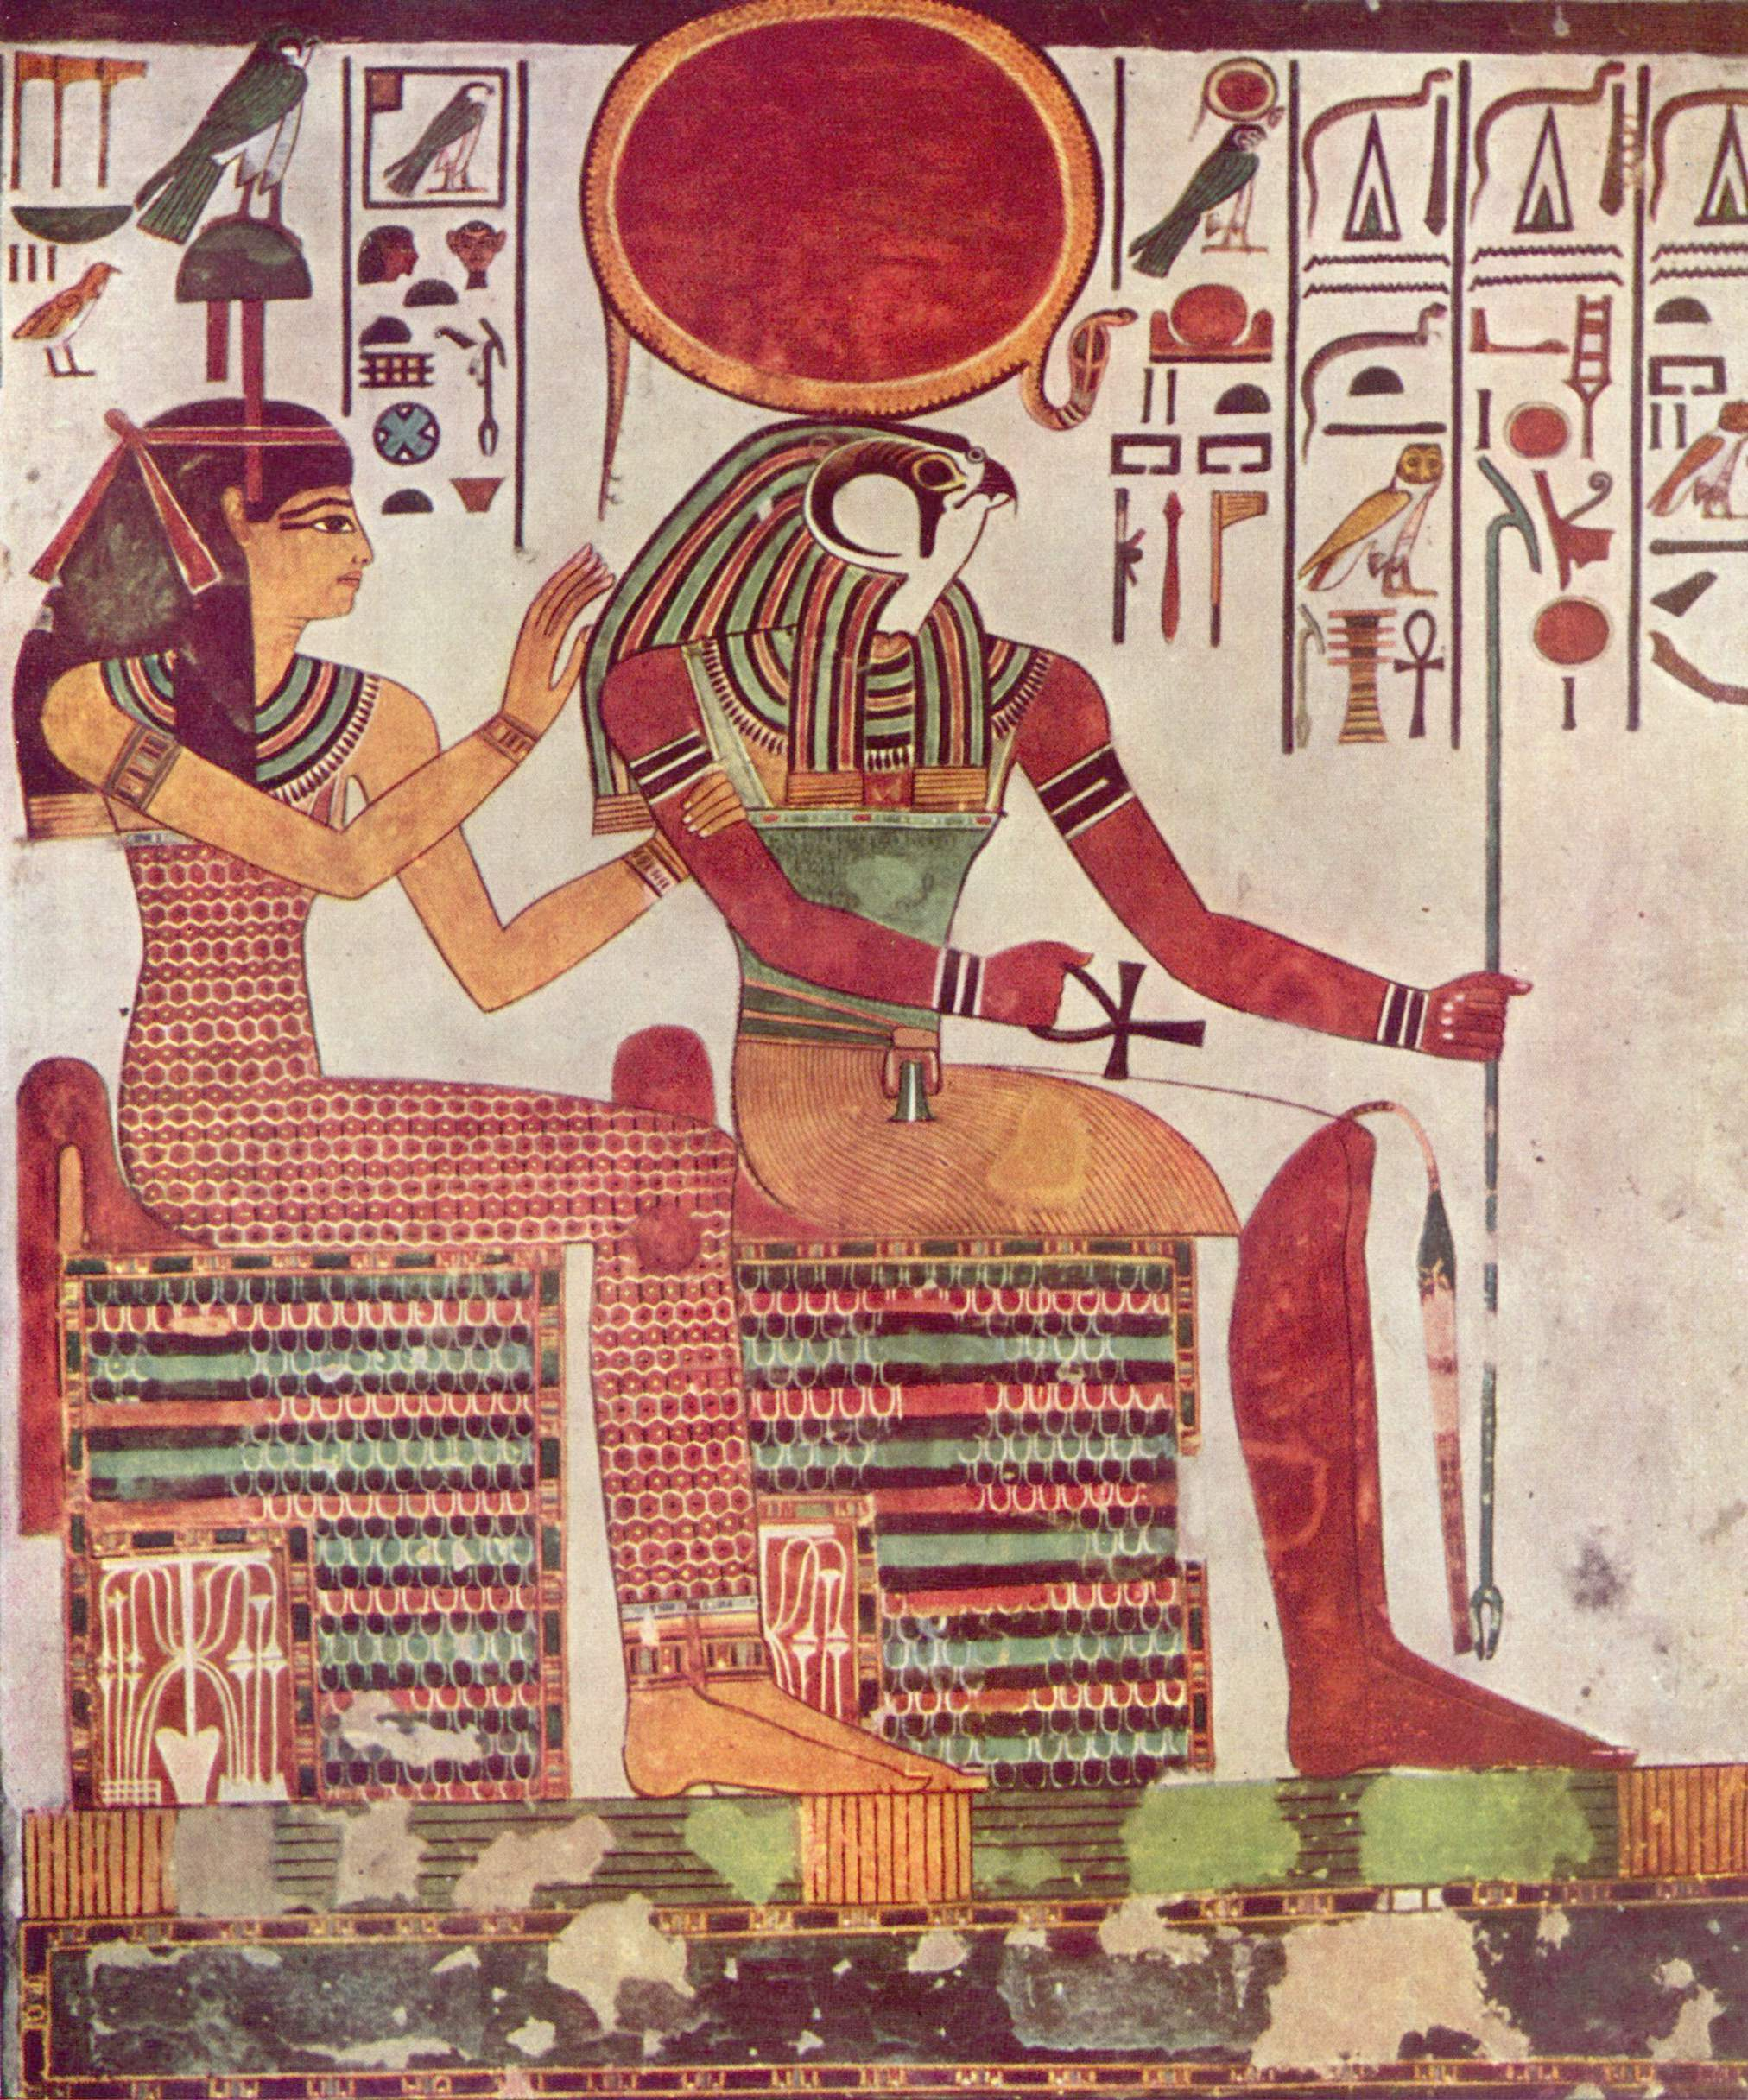
\includegraphics[height=5cm]{ra.jpg}
	\caption{historische Darstellung des Ra mit Sonnenscheibe}
	\label{ra}
\end{figure}
Die Augen wurden golden eingefärbt, um darzustellen, dass die Priesterin aus den Augen leuchtet. Die Haare sollten im Wind wehen und auffällig sein. Daher wurden sie weiß, sehr lang und mit vielen Strähnen gestaltet. Um den Hals gestalteten wir den auf Pharaonen- und Götterdarstellungen basierenden typisch ägyptischen goldenen Halsschmuck. Der Vogel-Arm wurde mit Federn versehen und die Klaue der eines realen Falken nachempfunden. Darüber wurde ein zerissener Ärmel aus Stoff gezeichnet, da flatternder Stoff gut mit der Vogel-Assoziation harmonisiert und weil es realistisch wäre, dass eine reale Person den Arm verstecken wollen würde.
\\Ursprünglich war für die Priesterin ein einärmliges Kleid geplant, aber nachdem verschiedene Konzepte für den Oberkörper ausprobiert wurden und sich für den goldenen geflügelten Skarabäus im Brustbereich entschieden wurde (ein weiteres bekanntes Symbol für Ra), wurde das Kleid verworfen und stattdessen ein Rock und Stofffetzen gewählt und der Ärmel am Halsschmuck 'befestigt'. Der rechte Arm war simpler in der Gestaltung und bekam den bekannten Goldschmuck, der auf vielen Darstellungen von Göttern, Göttinnen und Pharaonen zu sehen ist. Als Priesterin bekam sie einen Stab, da Stäbe und Szepter häufig mit Priestern assoziiert werden. Gewählt wurde eine verlängerte Version des Stabs der Könige. Der Gürtel sollte gewebt aussehen, um trotz Gold noch leicht auszusehen und brauchte wegen der Größe ein auffälliges Kopfteil. Der Rock bestand erneut aus flatterndem, himmelblauen Stoff, ebenfalls wegen der Vogel-Assoziation.

\newpage
\begin{figure}[H]
	\centering
	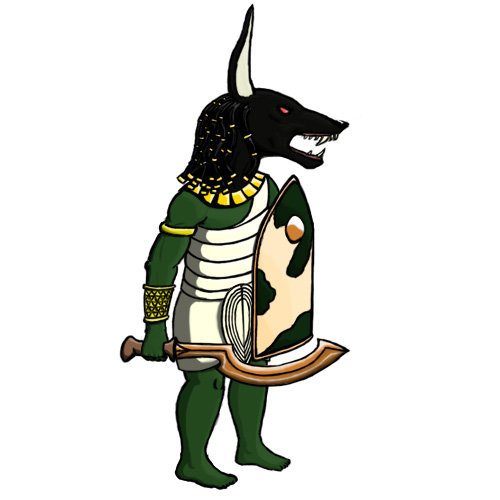
\includegraphics[height=7cm]{jackal.jpg}
	\caption{Der finale Schakalskrieger}
	\label{jackal}
\end{figure}
\subsubsection{Der Schakalskrieger}
Nach der Priesterin des Ra sollte eine etwas weniger fantastische Figur, die sich stärker an der historischen Realität orientierte und martialischer aussah in das Spiel eingebracht werden. 
\begin{figure}[H]
	\centering
	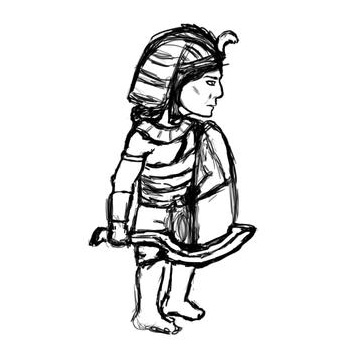
\includegraphics[height=5cm]{jackalalpha.jpg}
	\caption{Der frühe  Entwurf}
	\label{jackalalpha
	}
\end{figure} 
Da mit der Priesterin eine ägyptische Fernkämpferin existierte, war für die zweite ägyptische Figur ein Nahkämpfer vorgesehen. Daher orientierten wir uns in der Planung fortan am historischen Soldaten des dritten ägyptischen Zeitalters.
\\Der Soldat war anfangs als Mensch gezeichnet und trug ein vorher erwähntes Nemes als Kopftuch. Kopftücher dieser Art waren als Schutz gegen die Hitze recht üblich und sahen interessanter als einfache Haare aus. Zusätzlich zeichneten wir eine mehrschichtige Rüstung aus Leinen, inklusive eines auffälligen Lendenschurzes. In der Realität trugen Ägypter wegen der Hitze lange keine oder wenig Rüstung, Leinen wurde allerdings u. a. von Kriegern in Streitwägen benutzt. Das mit Kuhfell bespannte Holzschild war auffällig und von der Form her exotisch. Da es allerdings sehr groß war, zeichneten wir es im Gegensatz zu den Wikingern auf die vordere Hand (aus Sicht der Figur), da es sonst zu viel vom Körper verdeckt hätte. Als Waffe wurde ein sogenanntes Chepesch ausgewählt, eine exotische Waffe, die Eigenschaften einer Axt und eines Schwertes kombiniert und in der Moderne häufig mit Ägypten assoziiert wird. Sie war lange, aber nicht ausschließlich, eine Zeremonie-Waffe der Pharaonen und wurde, wie auch die anderen Waffen, etwas vergrößert gezeichnet. 
Danach wurden zunehmend fantastische Elemente hinzugefügt, um die Figur außergewöhnlicher aussehen zu lassen. Das Nemes bekam eine Schlange aufgesetzt, die als Zeichen der Königswürde von Totenmasken bekannt war. Wir zeichneten zusätzlich Schmuck um Hals und Arme die dem der Priesterin ähnelten, aber massiver aussahen. Dies stellte ein vereinendes Element unter den ägyptischen Figuren her, das weithin bekannt ist. 
\\Da der Kopf und die Figur insgesamt noch nicht aggressiv genug aussah, wurde der Kopf gegen einen Schakalskopf ausgetauscht, der Anubis nachempfunden war. Der ägyptische schakalsköpfige Gott der Einbalsamierung Anubis ist sehr bekannt und der Kopf gab dem Krieger ein 'beißerisches' Aussehen, etwas das dem originalen Entwurf gefehlt hatte. Nachdem mehrere Skizzen mit unterschiedlichem Kopfschmuck und Haaren erstellt wurde, wurde sich für schwarze Rhasta-Locken mit goldenen Bändern entschieden. Dies sorgte für einen außergewöhnliches Äußeres und funktionierte gut mit dem anderen Goldschmuck.
\\Da hier, im Gegensatz zu der Priesterin, der Arm mit dem Reif im Vordergrund steht, wurde die Armschiene stärker ausgearbeitet. Die Haut wurde dunkler gemacht, was einen starken Kontrast zu dem beigen Leinen erzeugte und der Figur ein unmenschlicheres Äußeres gab. Insbesondere sind Schakale mit Ausdauer und höheren Geschwindigkeiten assoziiert. Dies erleichterte die Erklärung, dass er mobiler war.
\newpage
\subsection{Animationen}\label{ani}
2D-Animationen funktionieren sowohl in Spielen, als auch in Filmen im Allgemeinen nach dem Daumenkino-Prinzip: Wenn man eine gewisse Zahl an Bildern (Frames genannt) pro Sekunde aneinander hängt, die Momente einer Bewegung zeigen, entsteht bei dem Betrachter das Gefühl einer Bewegung. Hierbei sind 24 Frames pro Sekunde optimal und kommen z.B. in Disney-Filmen zum Einsatz, zwölf sind auch für Menschen mit guten Augen nicht als einzelne Bilder erkennbar und sechs reichen, um den Eindruck von Bewegung entstehen zu lassen und kommen häufig bei Projekten mit geringem Budget, wie z.B. in den meisten 2D-Indie-Spielen zum Einsatz. %ändern
\\Aufgrund der begrenzten Mittel, sind die Animationen auch in diesem Spiel sechs bis zwölf Frames lang. Die Animationen sind eher simpel gehalten%...
, teilweise wurden sie allerdings aufpoliert, z.B. indem Licht und Schatten korrigiert, oder Muskulatur und sich bewegende Elemente wie Stofffalten neu gezeichnet wurden.\\
\begin{figure}[H]
	\centering
	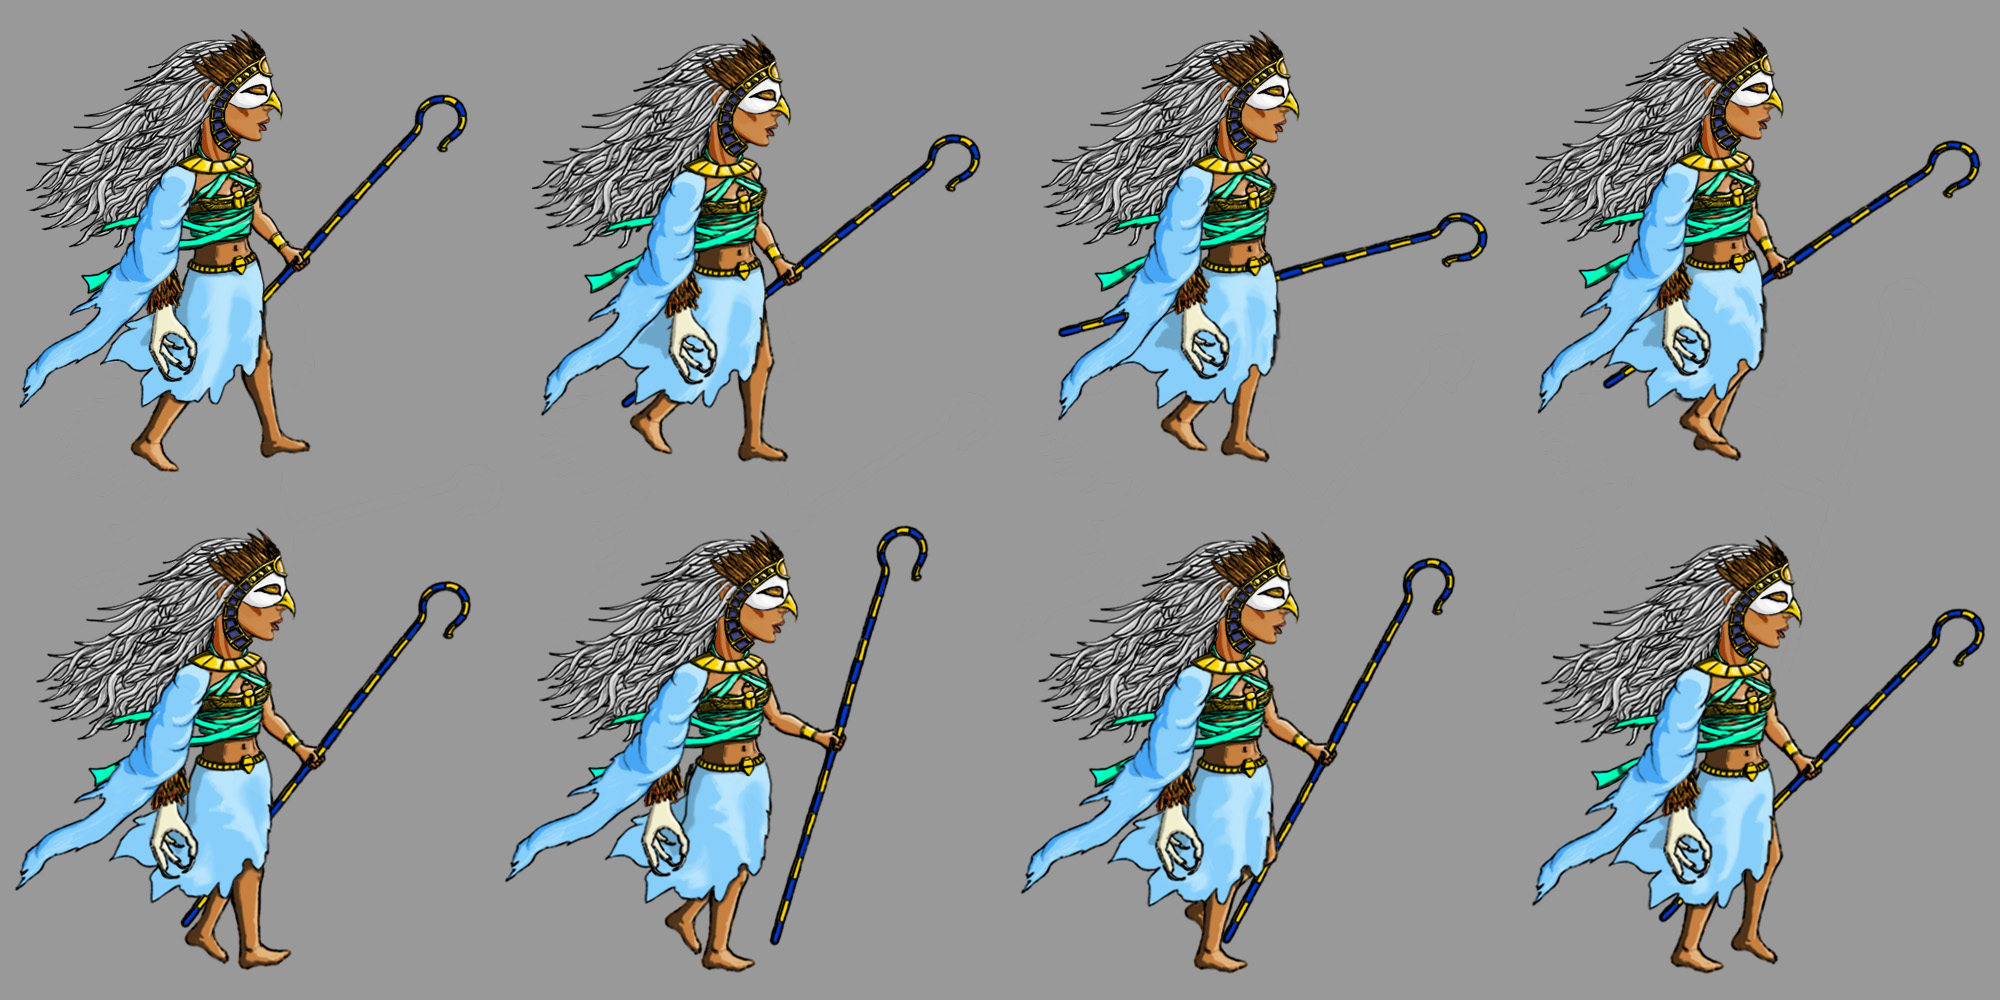
\includegraphics[height=5cm]{move.jpg}
	\caption{Ein Spritesheet für eine Laufanimation}
\end{figure}
Unsere Figuren bekamen Lauf- und Angriffsanimationen, wobei die Laufanimationen im Spiel solange wiederholt werden, bis die Figur ihr Ziel erreicht hat und die Angriffsanimationen einmal ausgeführt werden. Die Animationen wurden in sogenannten Spritesheets gespeichert, die in Unity dann wieder in einzelne Bilder zerlegt werden. Spritesheets sind mehrere Bilder, die in einem Bild gespeichert werden, sodass nicht jedes Bild einzeln geladen werden muss. Unity ist in der Lage, aus mehreren Bildern automatisch Animationen von einer Sekunde Dauer zu generieren, wobei an einigen Stellen die Animationen beschleunigt oder verlangsamt wurden, um bessere Ergebnisse zu erzielen. So wurden z. B. diverse Angriffsanimationen in eine langsamer abgespielte Aushol-Phase und eine schneller abgespielte Schlag-Phase aufgeteilt. Die Anbindung der Animationen an den Code geschieht dabei mithilfe des sogenannten Animator Controller, eines Zustandsautomaten, der für verschiedene Auslöser Animationen wechselt oder abspielt.
\begin{figure}[H]
	\centering
	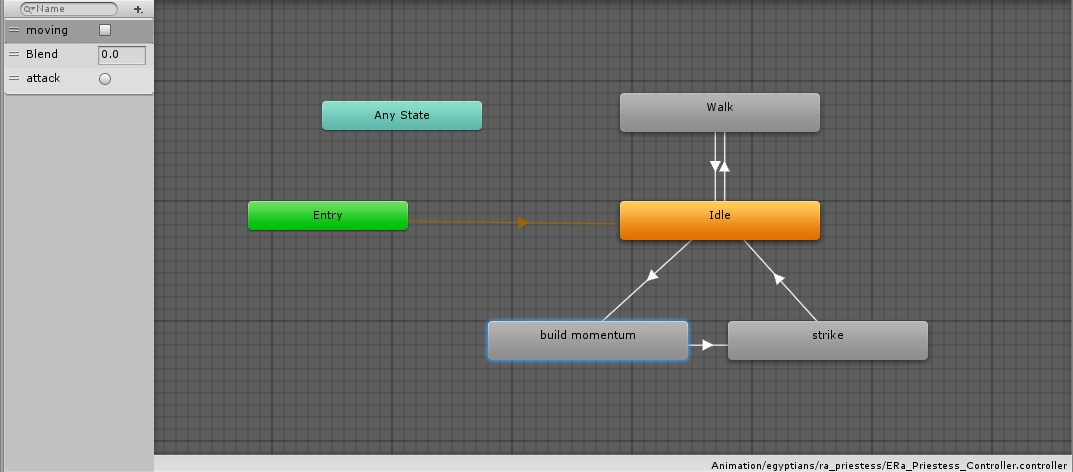
\includegraphics[height=5cm]{animator.jpg}
	\caption{Unity's Animator Contoller}
\end{figure}
\begin{figure}[H]
	\centering
	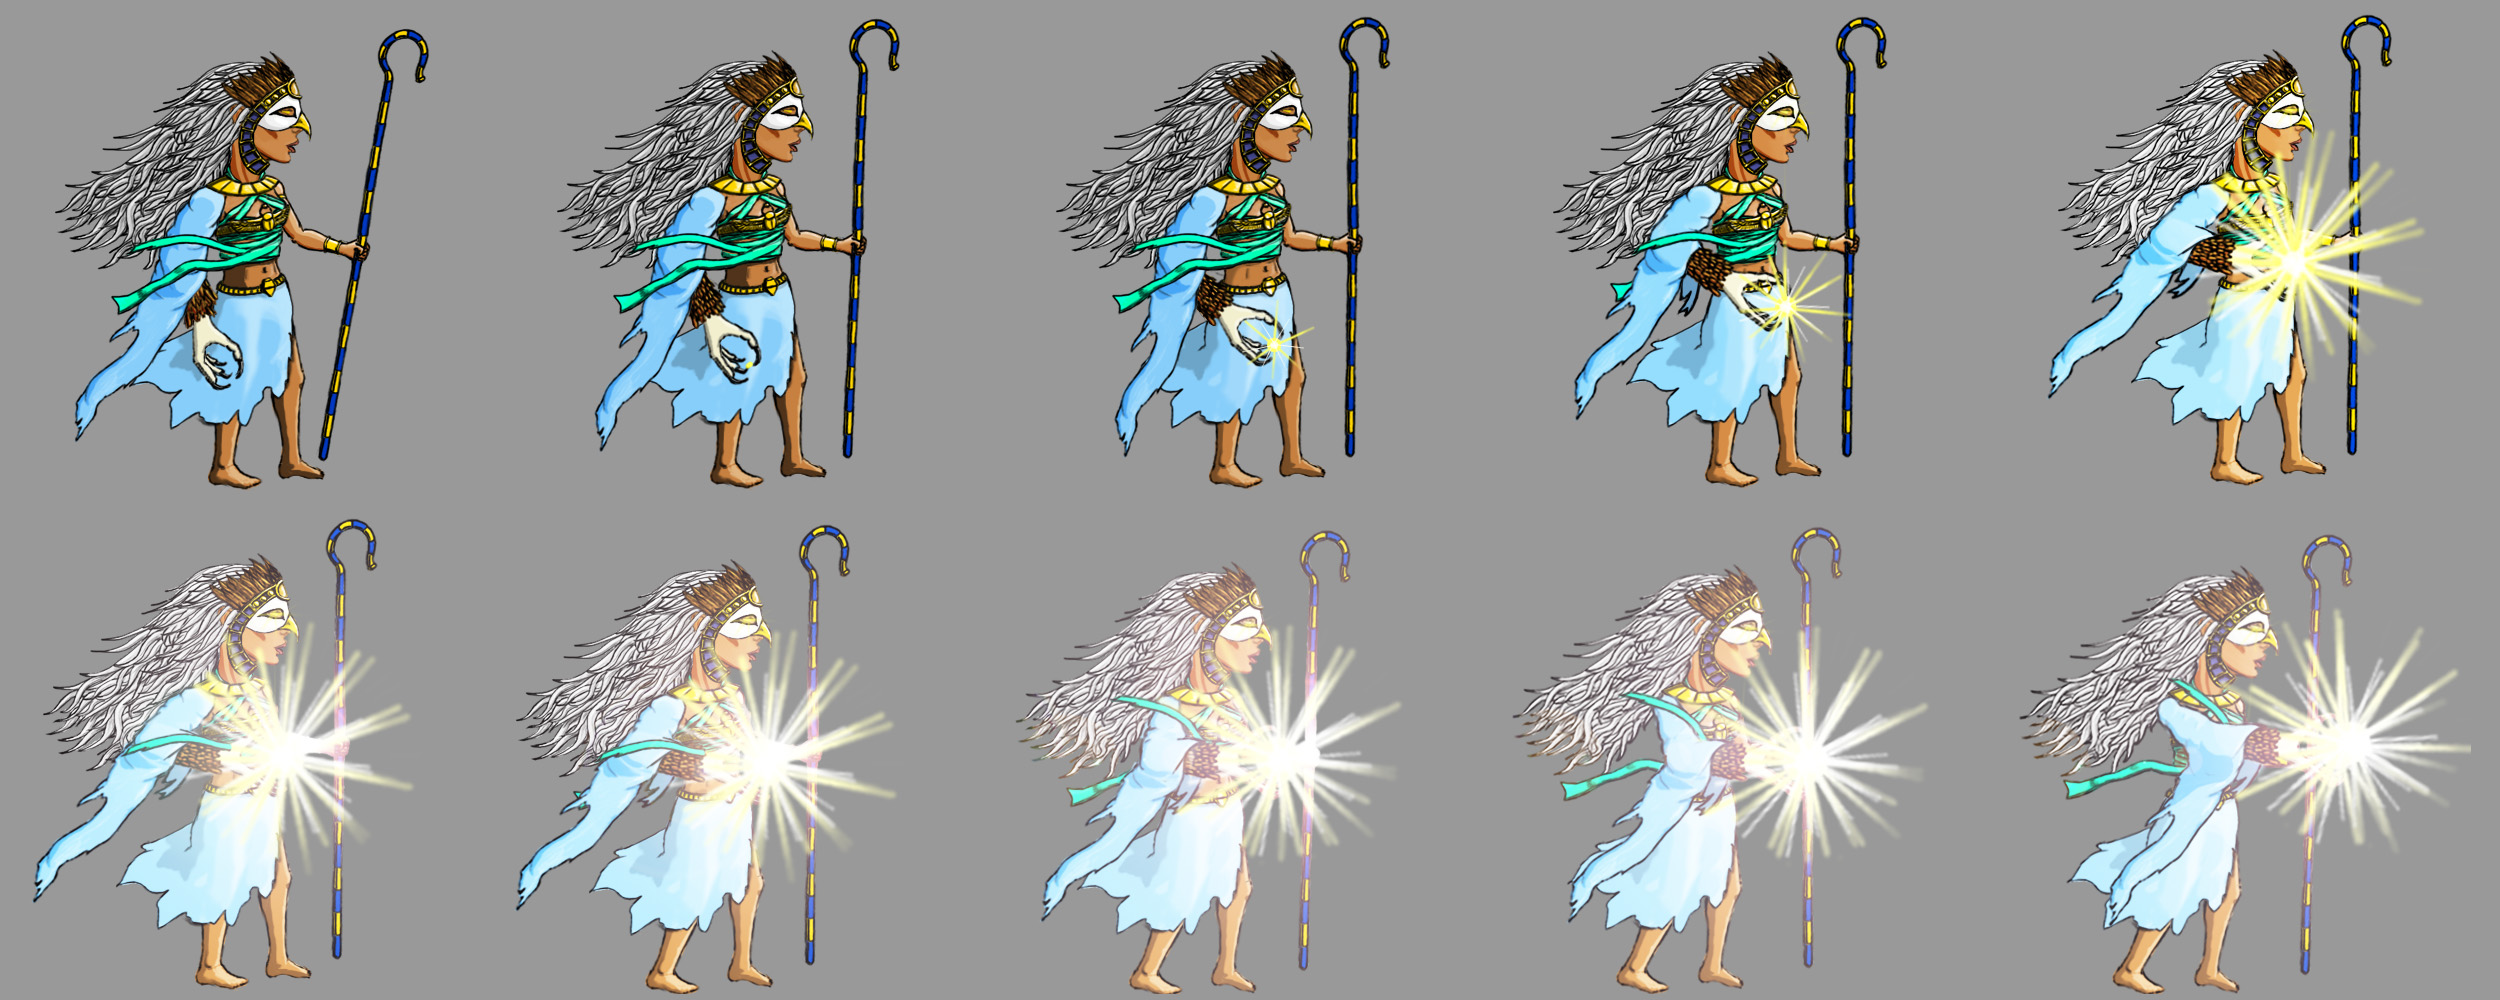
\includegraphics[height=5cm]{attack.jpg}
	\caption{Ein Spritesheet für eine Angriffsanimation}
\end{figure}
	
\section{Auswertung der Fragebögen}	Sowohl im Sinne einer objektiven Bewertung als auch um mögliche Fehler durch eine größere Anzahl von Tests zu ermitteln wurde das Spiel von einigen Personen getestet und deren Wertung mit einem Fragebogen erfasst. Da es Ziel war, im Gegensatz zu Pokemon Go möglichst zusätzliche Spielergruppen zu motivieren, das Spiel zu spielen, wurde nach der Entwicklung großer Wert darauf gelegt, möglichst unterschiedliche Testspieler zu finden und diese das Spiel ausprobieren zu lassen. Dabei war die schriftliche Befragung der Testpersonen in vier Themenbereiche gegliedert:
\begin{itemize}
	\item Unter 'Spielertyp' wurde die Nutzung von Computer und Smartphone sowie die Spielerneigung erfasst (Fragen 1-4). 
	\item Unter dem Oberbegriff 'User-Interface' wurde die Benutzerfreundlichkeit, die technische Umsetzung insbesondere bei der Steuerung sowie die Gestaltung der Menüs abgefragt (Fragen 5-10).
	\item Im Bereich 'Kämpfe' wurden deren Spaßfaktor und die strategische Tiefe sowie die grafische Gestaltung beurteilt (Fragen 11-15).
	\item Abschließend wurde die allgemeine Gesamtwertung unter den Aspekten Spielespaß, Verknüpfung der Spielelemente, längerfristiges Spielerinteresse sowie die Geeignetheit als mobiles Spiel erfragt (Fragen 16-20).
\end{itemize}
\subsection{Ermittlung und Einstufung des Spielertyps}
Im ersten Themenblock wurde die Computeraffinität und die Selbsteinschätzung des jeweiligen individuellen Spielertypus erfragt. Ergänzend wurden Alter und Geschlecht angegeben. Insgesamt haben 12 Testpersonen im Alter von 10 bis 68 Jahren das Spiel getestet und ihre Bewertung abgegeben. Davon waren vier weiblichen und acht männlichen Geschlechts. Dieses Datenmaterial bildet die Basis für die Untersuchung möglicher Korrelationen bei den weiteren Themenfeldern und ermöglicht am Ende ein Urteil, ob es gelungen ist, ein Spiel für breite Spielerschichten zu schaffen. 
\begin{figure}[H]
	\centering
	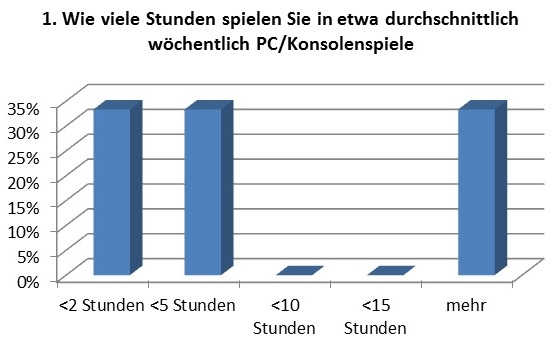
\includegraphics[width=1\textwidth]{table0.jpg}
\end{figure}
Die Ergebnisse der Frage 1 zeigen, dass die Testpersonen ein breites Spektrum von sehr versierten bis hin zu Spielern, die nur in sehr geringen Umfang spielen, repräsentieren. Auffällig ist, dass 10 der 12 Testpersonen weniger als 2 Stunden pro Woche auf ihrem Smartphone spielen (s. Frage 2).
\begin{figure}[H]
	\centering
	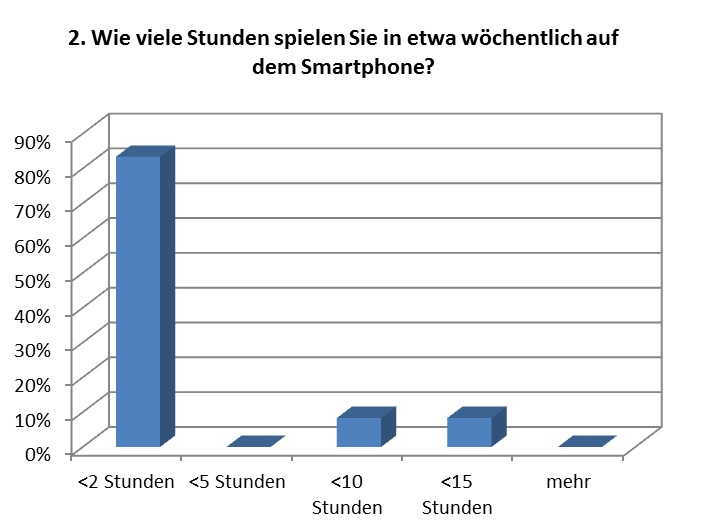
\includegraphics[width=1\textwidth]{table1.jpg}
\end{figure}
Die Mehrzahl der Testpersonen hat offenbar auch kein anhaltendes Interesse an Pokémon Go gehabt, da diese angegeben hatten, dies zweitweise intensiv gespielt zu haben. Dies macht uns in Bezug auf deren Feedback auf unser Spiel besonders neugierig. Nur zwei Personen (beide weiblich) geben an, regelmäßig zwischen 5 und 15 Stunden pro Woche auf dem Smartphone zu spielen. 
Eine breite Streuung ergab sich bei der Frage, ob eher einfache oder eher komplexe Spiele bevorzugt würden. Dabei bevorzugen 50\% 'eher einfach' zu erlernende Spiele, aber auch insgesamt 42\% 'eher komplexe' oder 'komplexe' Spiele. 
\begin{figure}[H]
	\centering
	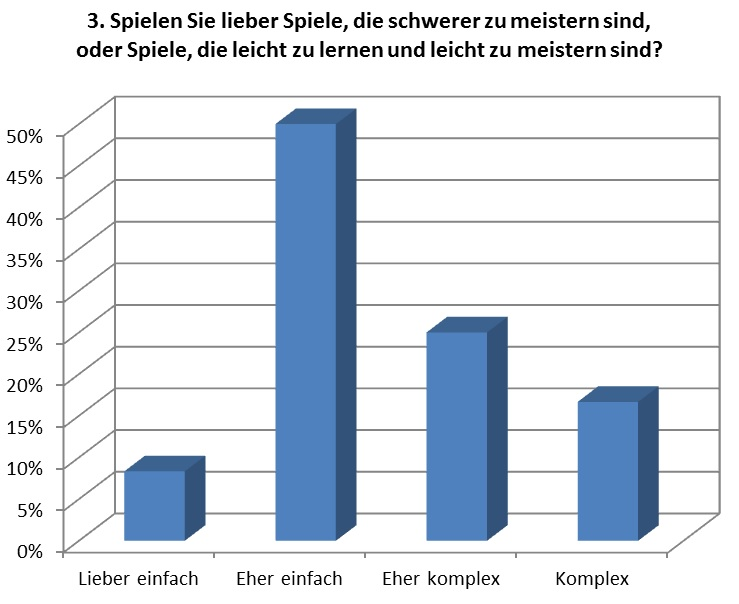
\includegraphics[width=1\textwidth]{table2.jpg}
\end{figure}
Die Ränder der Verteilung  waren stärker ausgeprägt bei der Frage nach der Anzahl der Rollenspiele, die bisher gespielt wurden. Hier hat 1/3 der Befragten in der Vergangenheit mehr als acht Rollenspiele gespielt, aber immerhin 42 % bislang noch keins gespielt?
\begin{figure}[H]
	\centering
	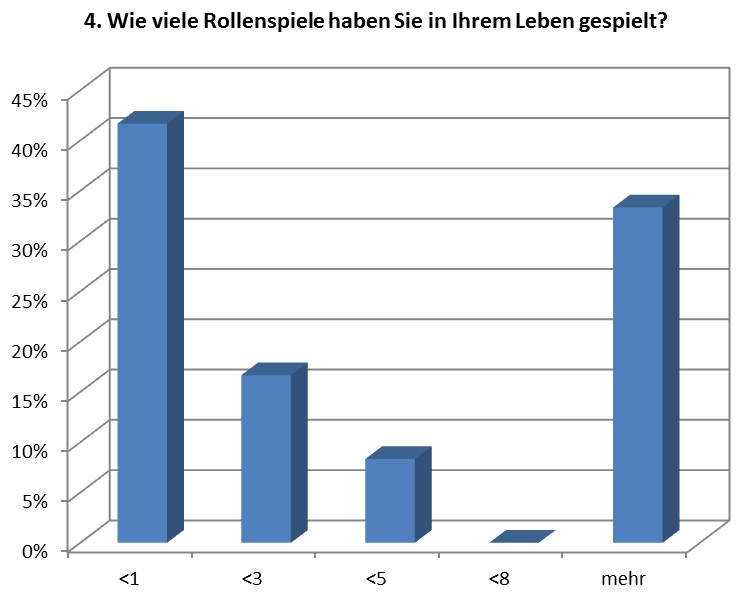
\includegraphics[width=1\textwidth]{table3.jpg}
\end{figure}
Gerade im Hinblick auf die gewünschte breite Streuung der Testpersonen ist die Korrelation der Fragen bei den unterschiedlichen Probanden interessant. In der nachfolgenden Tabelle zeigt sich, dass insbesondere die Intensiv-Spieler mit 15 Stunden und mehr wöchentlich 'eher komplexe' bzw. 'komplexe' Spiele bevorzugen und auch die größere Erfahrung bei Rollenspielen ausweisen.  Im Gegenzug gibt es ein Spektrum von Personen, die so gut wie nie digitale Spiele spielen und noch nie ein Rollenspiel gespielt haben (siehe z.B. die drei weiblichen Testspieler C, H und J und der 66 jährige männliche Spieler K, Antwort 4a) bis zu echten 'Gamern' mit sehr hoher Spielerfahrung (siehe die 'mittel-alte' Gruppe im Alter von 20 bis 30 Jahren aus den Spielern D, E, F und G; Antwort 1e). Die Nutzung des Smartphones als Spielgerät erfolgt (nach Abflauen des Pokemon Go-Hypes) überwiegend in geringem Umfang. Interessanterweise sind die beiden intensiveren Nutzer des Smartphones in der Gruppe der Über-60-Jährigen zu finden.
\begin{figure}[H]
	\centering
	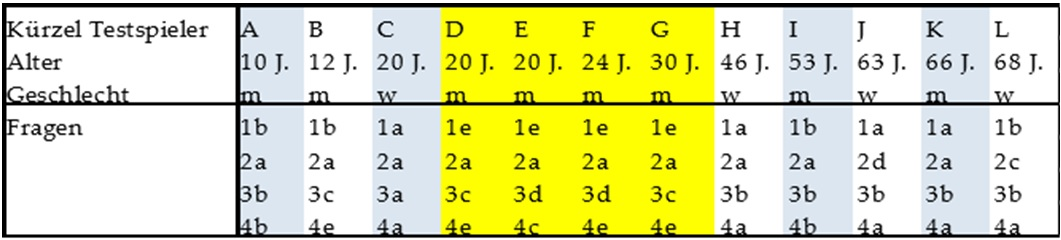
\includegraphics[width=1\textwidth]{testspieler.jpg}
\end{figure} 
Unterm Strich zeigt sich, dass die Gruppe der Testpersonen die gewünschte breite Streuung von verschiedenen Spielertypen mit unterschiedlichem Nutzerverhalten und Erfahrungen aufweist.  Durch diese sehr vielfältige Gruppe von Testern wird es besonders spannend, herauszufinden, wem unser Prototyp Spaß macht und welchen Personen nicht und wer welche Verbesserungsideen vorschlägt.
\newpage
\subsection{Bewertung des User-Interface}
Da eine möglichst breite Ansprache unterschiedlicher Spielertypen erfolgen sollte, sollte der Einstieg in das Spiel möglichst einfach erfolgen. Gerade vor dem Hintergrund, dass das Spiel als Handygame konzipiert wurde, ist zu erwarten, dass Spieler hier nicht die Geduld bzw. Zeit mitbringen, sich auf einen langwierigen Einstieg einzulassen. 
\begin{figure}[H]
	\centering
	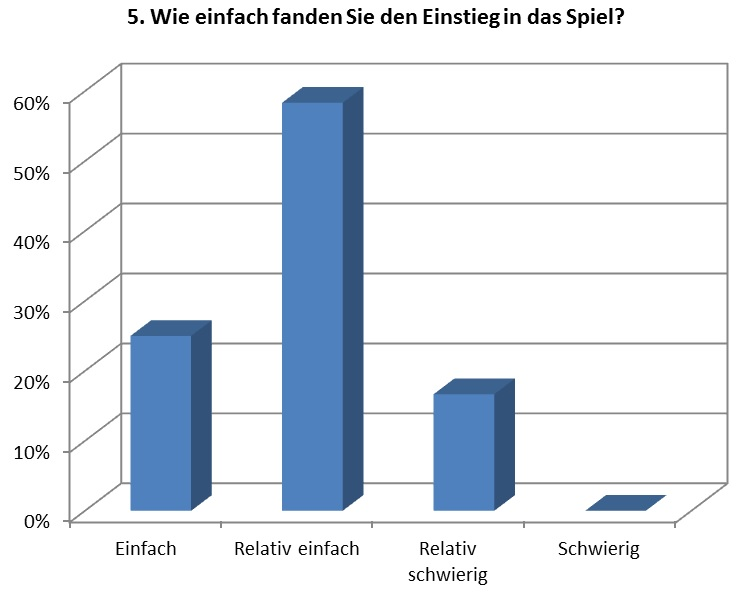
\includegraphics[width=1\textwidth]{table4.jpg}
\end{figure}
Mit drei von zwölf Testpersonen fanden 25\% den Einstieg als 'einfach' und weitere sieben Personen (58\%) als 'relativ einfach'. Nur zwei Personen empfanden den Einstieg als 'relativ schwierig' und keiner als 'schwierig'. Somit dürfte dieser Zielsetzungspunkt verwirklicht worden sein. 
Dies bestätigen auch die Erfahrungen der Handhabung der Menüs. Diese empfanden 33\% als 'intuitiv' und weiter 58\% nach der Eingewöhnungszeit als 'gut'. Nur eine einzige Testperson empfand die Menüs als 'gewöhnungsbedürftig. 
\begin{figure}[H]
	\centering
	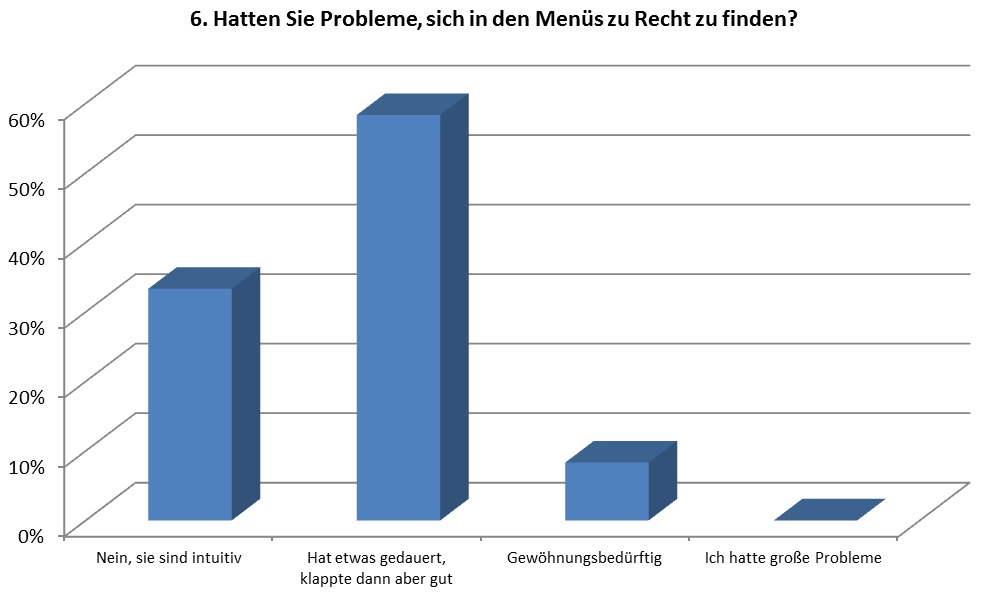
\includegraphics[width=1\textwidth]{table5.jpg}
\end{figure}
Noch besser wurde die Steuerung in den Menüs bewertet, die 2/3 der Testpersonen als 'gut, hat problemlos geklappt' einstuften. 'Ganz okay, kleinere Probleme' hatten hier 25\% und nur eine Testperson hatte 'häufig Probleme' und keiner beurteilte diese als 'schlecht, andauernde Probleme'.
\begin{figure}[H]
	\centering
	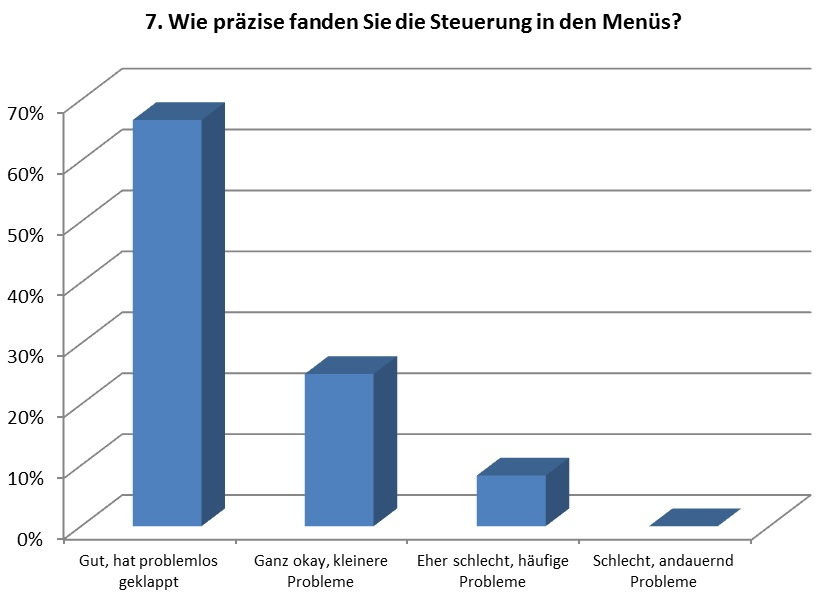
\includegraphics[width=1\textwidth]{table6.jpg}
\end{figure}
Positiv schnitt auch die Steuerung auf dem 'Map Screen' ab. Diese wurde von der Hälfte als 'sehr intuitiv eingestuft, weitere 42\% bewerteten diese als 'intuitiv nach einer kleinen Gewöhnungsphase'. Nur eine Person beurteilte diese als 'sehr kompliziert/unpraktisch' mit der niedrigsten Beurteilung.
\begin{figure}[H]
	\centering
	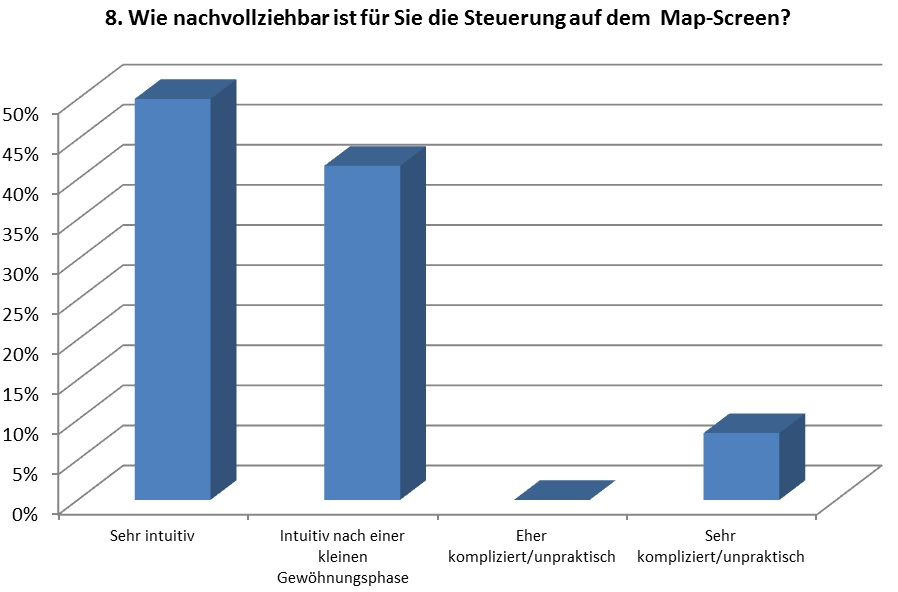
\includegraphics[width=1\textwidth]{table7.jpg}
\end{figure}
Weitreichende Zustimmung fand die Gestaltung des Party- und Quest-Menüs, denn dies wurde von allen Testpersonen als gut, wenn auch in graduellen Abstufungen bewertet. 'Sieht sehr gut aus' beurteilten 1/3 und 'sieht gut aus'  weitere 50\%. Rund 17\% urteilten in der Kategorie 'sieht eher gut aus', während keine der Testpersonen im negativen Wertungsbereich von 'sieht eher schlecht aus' bis 'ist sehr hässlich'  urteilte.
\begin{figure}[H]
	\centering
	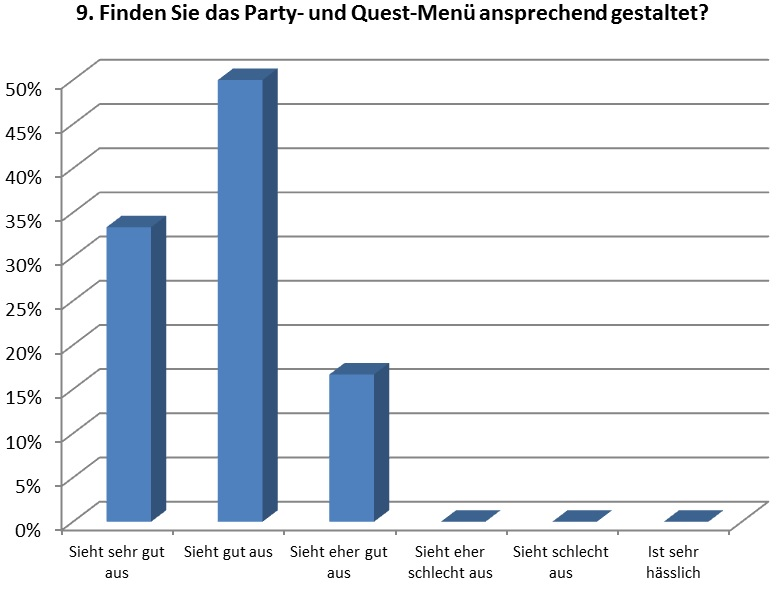
\includegraphics[width=1\textwidth]{table8.jpg}
\end{figure}
Als Wünsche oder Kommentierung zum Map- oder Party-Menü (Frage 10: Haben Sie andere Anmerkungen oder Wünsche zum Map- oder zum Party-Menü?) wurden von den Testpersonen ganz überwiegend Wünsche im Hinblick auf eine Erweiterung des Spiels bzw. der -funktionen ausgesprochen: ++ \textit{“Mehrspieler-Modus wäre gut“}  ++ \textit{„Buttons im Artwork des Spiels designen; Items ablegbar machen, ohne ein weiteres diesen Typs zu besitzen“} ++ \textit{„Alles gut organisiert/konzipiert. Einziger Wunsch: Erklärung wie man Figuren auswählt und wie man Items den Figuren zuordnen kann. Außerdem: Möglichkeit, Gegner mit seinen Fähigkeiten anzuschauen, kreieren“} oder ++ \textit{„Ich würde die Orientierung auf dem Map-Screen an der Orientierung des Smartphones ausrichten.“}
Bis auf einen vereinzelten Fall in den jeweiligen Fragen beurteilten die Testpersonen die technische Handhabung und die Gestaltung der Benutzerschnittstelle positiv bis sehr positiv. Wünsche wurden vor allem im Hinblick auf die Erweiterung der Spielfunktionen geäußert.
\subsection{Gestaltung der Kämpfe}
Über 90\% der Testpersonen antworteten auf die Frage 11 'Machen Ihnen die Kämpfe Spaß?' mit 'Ja sehr'  (42\%) oder 'Ja meistens' (50\%). Eine einzige Probandin fand die Kämpfe eher langweilig. Diese Testperson (20 Jahre, weiblich) kann aufgrund ihres Spielprofils als wenig aktiv und auch wenig erfahren eingestuft werden und hat auch hier wohl als einzige keine Freude an den Kämpfen entwickeln können. 
\begin{figure}[H]
	\centering
	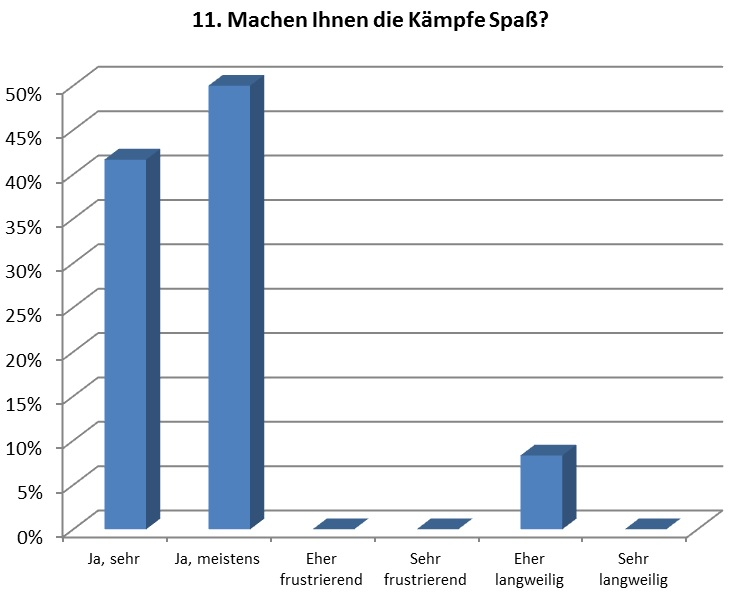
\includegraphics[width=1\textwidth]{table9.jpg}
\end{figure}
Einheitlicher war das Bild dann wieder bei der Beurteilung von Grafik und Stil der Kämpfe. 16,6\% der Testpersonen fanden diese 'sehr gut' und weitere 2/3 aller Teilnehmer 'gut', sowie zwei noch 'ganz gut'. Negativerer Beurteilung in den schlechteren Wertungsstufen fanden sich nicht, so dass unterm Strich der Mittelwert aller Beurteilung bei 'gut' liegt.
\begin{figure}[H]
	\centering
	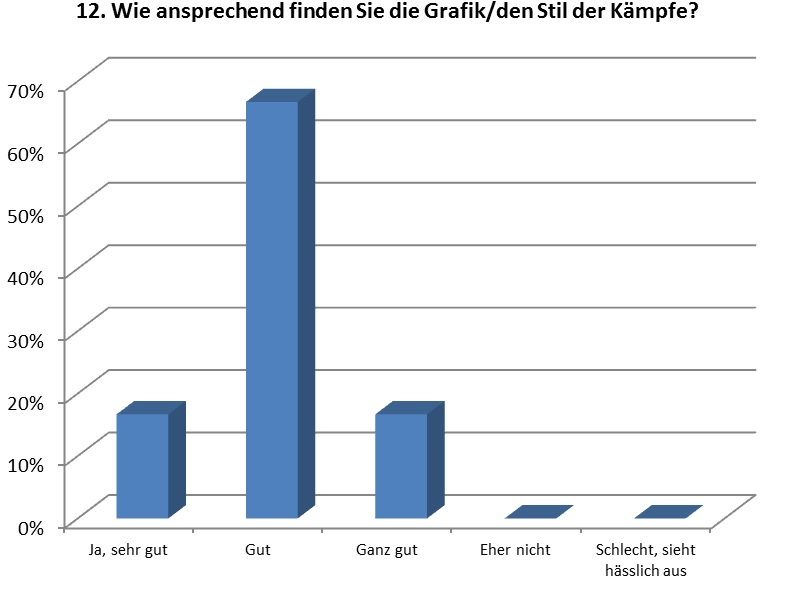
\includegraphics[width=1\textwidth]{table10.jpg}
\end{figure}
Im direkten Vergleich zu dem eher kindlicheren Stil von Pokémon fanden wiederum 64\% der Teilnehmer den in unserem Spiel verwandten Stil besser. Nur eine Testperson bevorzugte den Pokemon-Stil, während eine Person sich zu der Frage überhaupt nicht äußerte und zwei angaben, dass dies ihnen 'recht egal' sei. 
\begin{figure}[H]
	\centering
	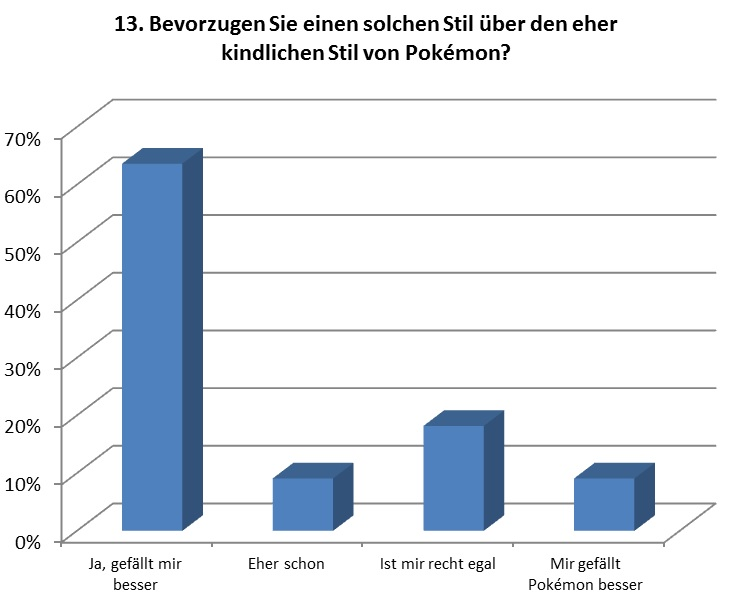
\includegraphics[width=1\textwidth]{table11.jpg}
\end{figure}
Wie intensiv sich die Testpersonen mit den Kämpfen beschäftigt haben, haben wir nachfolgend in Frage 14 'Haben die Kämpfe Tiefe? Denken Sie über Ihre Züge nach?' untersucht. Hier zeigte sich dass die ganz große Mehrheit die strategischere Ausrichtung des Spiels aufgreift: 42\% der Befragten denken 'häufig' über ihre Züge nach und ebenfalls 42\% gemäß der nächsten Kategorie 'gelegentlich'. 'Eher selten' oder 'Nie' tat dies keiner, während zwei Personen angaben 'fast nie' über ihre Züge nachzudenken. Dabei handelt es sich bei beiden um 'Intensiv-Spieler' mit großer Rollenspielerfahrung, denen vermutlich ihr Handeln in 'Fleisch und Blut' übergegangen ist. 
\begin{figure}[H]
	\centering
	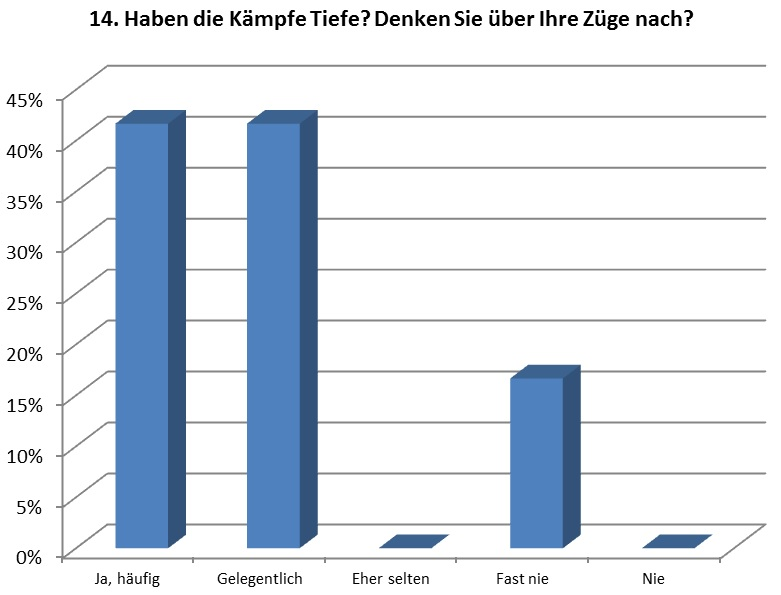
\includegraphics[width=1\textwidth]{table12.jpg}
\end{figure}
Mit Frage 15 'Haben Sie Anmerkungen oder Verbesserungsvorschläge für die Kämpfe?' wurde dieser Themenbereich abgeschlossen. Zweimal wurde erwähnt, dass nicht kenntlich ist, wer am Zug ist: ++  \textit{„Wer kämpft ist unklar“} ++ \textit{„Anzeige, was gerade passiert wäre hilfreich, und wer gerade dran ist.“} Da die Figuren durch die Anzeige (hellerer) Zugfelder kenntlich gemacht werden, könnte hier die Ursache darin liegen, dass aufgrund der Bewegung draußen und möglicher Sonneneinstrahlung der Kontrast zu gering ist, wie nachfolgendes Statement untermauert. \textit{„Hintergrund des Bildschirms beim Kampf finde ich zu dunkel. Man muss Handy sehr hell einstellen (Akkuverbrauch).“}\\
Eine weitere Gruppe hat Erweiterungen vorgeschlagen: ++  \textit{“Man könnte noch mehr Elemente in die Karte der Kämpfe einbauen (neben den Felsen).“} ++ \textit{„Relativ einfach nach kurzer Zeit“} ++ \textit{”I found it impossible to beat the bosses at first. I loved the fireballs. It might be nice to have more and other visually interesting weapons. But I thought it was fun.”} Während andere die vorhandenen unterschiedlichen Spielelemente ausdrücklich lobten: ++ \textit{„Spiel macht noch mehr Spaß, als die Quests dazukamen- Damit wurden längerfristige Ziele gesetzt, so dass Spielmotivation erhöht wurde. Man spielt also länger.“} ++ \textit{„Sehr gut finde ich unterschiedliche Kämpfer mit unterschiedlichen Funktionen, die Kämpfe interessanter gestalten.“}
\\
\\
Zielsetzung waren sowohl mit einer 'erwachseneren' Darstellung als auch durch eine bessere Spieltiefe und die Integration strategischer Element die Spieler besser anzusprechen und so zu veranlassen, sich intensiver mit dem Spiel zu befassen und sie dadurch längerfristig zu binden. Sowohl die Spielidee in den Kämpfen als auch die Grafik wurden von den Testpersonen in hohem Maße positiv bis sehr positiv bewertet. Bei der Spieltiefe denken zwei sehr intensive Spieler wenig über die Kämpfe nach, alle anderen aber setzen sich durchaus intensiv mit dem Spielgeschehen auseinander. Zusammenfassend zeigt sich, dass sich die Testpersonen sowohl von der Grafik als auch der Spielidee in den Kämpfen positiv angesprochen fühlen.
\newpage
\subsection{Allgemeine Gesamtbewertung des Spiels}
Im vierten Block der Umfrage sollten die Testpersonen das Spiel insgesamt bewerten. Zunächst wurde mit Frage 16 'Macht Ihnen das Spiel Spaß? Wenn Nein, warum nicht?'  die Spielfreude ermittelt.  Mit 58\% beurteilte mehr als die Hälfte der Probanden die Spielfreude mit der höchsten Stufe ('Ja, sehr) gefolgt von 48\% in der zweitbesten Beurteilung ('Meistens'). Da es keine schlechteren Bewertungen gab, entfiel in dieser Frage auch die Kommentierung, auf die wir insgesamt bei Frage 20 zurückkommen werden. 
\begin{figure}[H]
	\centering
	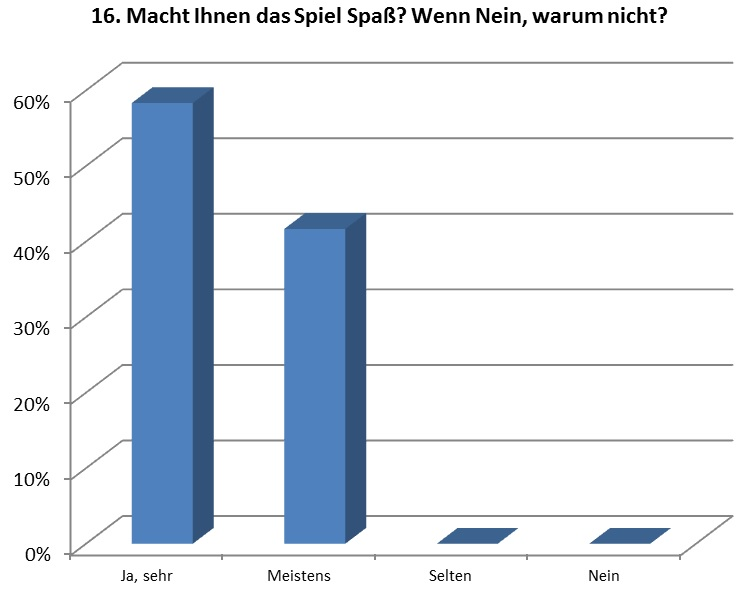
\includegraphics[width=1\textwidth]{table13.jpg}
\end{figure}
Da für das Gefühl des Spielflusses das Zusammenwirken der einzelnen Elemente entscheidend ist, wurde diese in Frage 17 von den Testpersonen beurteilt. 92\% der Testpersonen beurteilten auch hier das Spiel mit der Bestnote 'Gut, fühlt sich gut verknüpft an'. Lediglich eine Testperson urteilte in der nächsten Notenstufe mit 'Ganz gut', einzelne Elemente  greifen nicht ineinander', kommentierte hier jedoch nicht, wo er einzelne Brüche sah. Keine der Testpersonen urteilte mit den weiteren negativeren Notenstufen, so dass die Verknüpfung der Elemente und der Spielfluss wohl gelungen zu sein scheint. 
\begin{figure}[H]
	\centering
	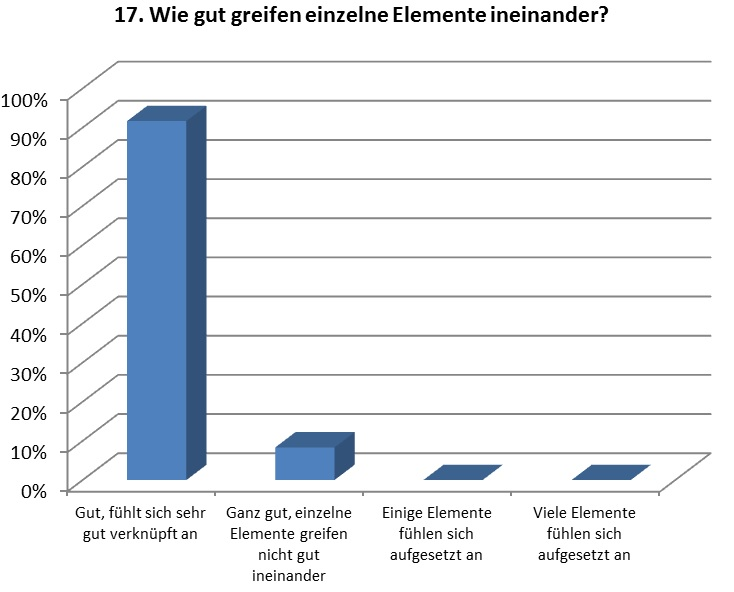
\includegraphics[width=1\textwidth]{table14.jpg}
\end{figure}
Die Aufgabenstellung war es einen Prototyp zu entwickeln, der AR-Elemente verwendet, einen leichten Einstieg bietet und das Potenzial hat, langfristig Spaß zu machen und zu fesseln. Nach der Gesamtbewertung von Spielspaß und –fluss sollte die Bindung an das Spiel und die längerfristige Tragfähigkeit des Spiels in Frage 18 'Könnten Sie sich vorstellen, das Spiel über einen  längeren Zeitraum zu spielen, wenn mehr Inhalte existieren würden oder das Spiel etwas besser ausbalanciert wäre?' ermittelt werden. Alle 12 Testpersonen konnten sich dies vorstellen und urteilten mit der besten Wertungskategorie 'Ja, das Prinzip ist gut und könnte auf längere Zeit fesseln. Die unter Frage 20 folgenden Kommentierungen zeigen die Gründe für die durchweg positive Beurteilung  
\begin{figure}[H]
	\centering
	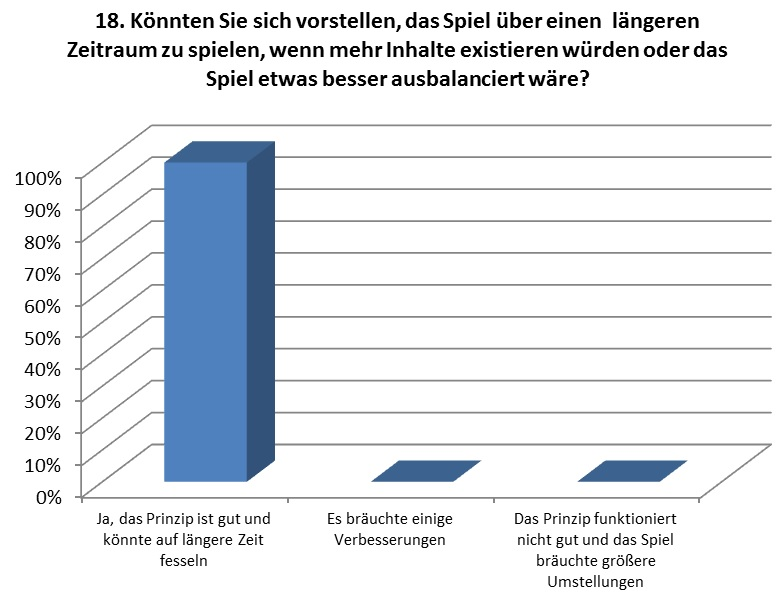
\includegraphics[width=1\textwidth]{table15.jpg}
\end{figure} 
Gerade vor dem Hintergrund, dass die Testpersonen über einen sehr unterschiedlichen Background  verfügen und die wenigstens intensive Handygamer sind, ist dies ein schöner Erfolg. Doch 'funktioniert das Spiel auch gut als mobiles Spiel? Kann man es gut unterwegs spielen, z.B. als Zeitvertreib auf dem Weg zum Einkaufen?' lautet Frage 19, um den mobilen Nutzwert, der speziell durch das Geo-Prinzip begründet wird, zu ermitteln. Auch hier waren 75\% der Testpersonen der Ansicht, dass das Spiel uneingeschränkt dafür geeignet ist und nur 25\% sahen leichte Einschränkungen, da das Spiel eine  entsprechende Konzentration beanspruche. Größere Einschränkungen oder das völlige Versagen als mobiles Spiel sah keine der Personen. 
\begin{figure}[H]
	\centering
	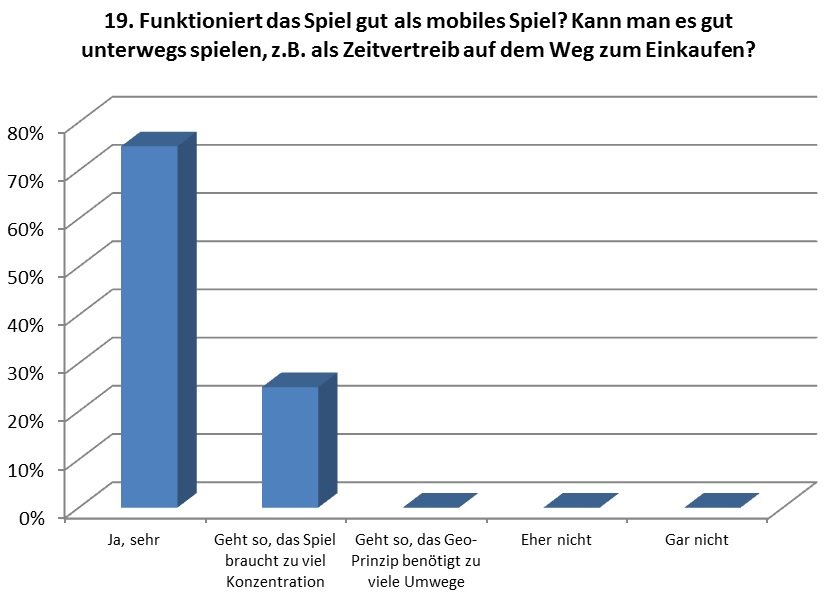
\includegraphics[width=1\textwidth]{table16.jpg}
\end{figure}
Mit Frage 20 'Welchen Gesamteindruck haben Sie von dem Spiel? Würden Sie bestimmte Elemente/Aspekte ändern? Haben Sie noch andere Anmerkungen? ' wurden die Testpersonen zu einer umfassenden Kommentierung gebeten.\\
Obwohl die große Mehrzahl den Spieleinstieg 'einfach' oder 'relativ einfach' fanden, wurde eine einleitende Erläuterung vorgeschlagen: ++ \textit{„Es wäre gut, wenn am Anfang ein Tutorial wäre. Entweder könnte eine Stimme erklären, was man tun muss, oder es könnten Sprechblasen (mit Pfeilen) erscheinen, in denen steht, was man tun muss. An sich hat mir das Spiel gut gefallen. Die Figuren gefielen mir gut.“} ++\textit{“ Kritik: Die Auswahl der Figuren ist nicht selbsterklärend, könnte für Anfänger erklärt werden, Erste Schritte sollten grundsätzlich erklärt werde.“} Zwar traten die Probleme vereinzelt und bei  wenig PC-spielaffinen Testpersonen auf, doch ist dies gerade für diese Zielgruppe ein wichtiger Hinweis. Für die meisten auch der weniger spielerfahrenen Personen war der Einstieg jedoch intuitiv möglich: ++ \textit{“Easy to get into, but lots to learn” ++ „Das Spiel ist sehr leicht zu lernen, wird aber durch die Konzeption nicht langweilig, da – das Levelsystem Anreize setzt sich selbst fortzuentwickeln und auch mal starke/übermächtige Gegner anzugreifen – unterschiedlich besetzte Teams unterschiedliche Strategien ermöglichen (Nahkampf/Fernkampf  mit Flucht und Distanz) – Items Anreize setzen, eigene Charakter zu erstellen, weiterzuentwickeln und so die Spielfiguren vom gleichen Typ zusätzliche Variationen bieten.“}\\
Die Vielspieler hingegen schlagen hier Erweiterungen und insbesondere einen Multiplayer-Modus vor: ++ \textit{„Gutes Design, Langzeitmotivation (noch) gering, da es noch keinen Multiplayer gibt.“} ++ \textit{„Ein Multiplayer-Modus (Kampf gegen andere Spieler) könnte dazu beitragen, die Langzeitmotivation zu verbessern.“} ++ \textit{„Komplexität ist für ein Mobile-Spiel angemessen und läuft recht stabil (Slowdowns können auch an meinem Gerät liegen). Da Pokemon Go einen Geospielehype ausgelöst hat, könnte so ein Spiel ebenfalls erfolgreich sein, wenn mehr Inhalte vorhanden sind. Für eine offizielle Veröffentlichung fehlen noch Designkniffe wie Soundeffekte, um das Spiel ansprechender zu machen (z. B. Angriff- und Treffersounds).“}
\\Durch die Bank positiv kommentiert wurde das optische Design: ++ \textit{„It's a brilliant design.“} ++ \textit{„Optisch finde ich das Spiel deutlich ansprechender als Pokemon Go, da für mich die Pokemon-Figuren eher für ein sehr junges Publikum designed sind. Die Figuren hier sind interessanter.“} ++ \textit{„Gestaltung der Figuren finde ich sehr gut und optisch viel ansprechender, als bei Pokemon Go.“} ++ \textit{„Interessant sind die unterschiedlichen Fähigkeiten der Figuren. Insbesondere die Priesterin, die aus weiter Entfernung den Gegner mit dem Feuerball schädigt, ist cool.“} 
\\
Ebenso wie der Spielfluss und die Konzeption: ++ \textit{„Die Kämpfe sind in Bezug auf Gewinne und Verluste gut ausbalanciert, so dass man nicht immer gewinnt, aber auch als 'Absolute beginner' Chancen hat, die Gegner zu zerstören und zusätzliche Waffen zu erhalten was wiederum motiviert, weiterzuspielen. Schön ist, dass die Gegner sehr schnell agieren, so dass man eigentlich die meiste Zeit selbst spielt und nicht warten muss“} ++ \textit{„Die Kämpfe sind machbar, nicht zu schwierig und nicht zu leicht. Die Figuren sehen gut aus. Hat Spaß gemacht, draußen die Figuren zu suchen.“}
\\
Und auch bei weiteren Teilnehmern spielt der Geospielgedanke eine wichtige Rolle: ++ \textit{„Gut durchdachtes Spielekonzept, das die Spieleanreize aus leistungsstärkeren PC-Spielen mit der 'Realität' vor Ort verknüpft und in mobiler Variante umsetzt. Man kann so die Wartezeit bspw. an der Bushaltestelle gut überbrücken und immer wieder nachschauen, welche Gegner an bestimmten Orten sind, an denen man häufiger ist, aber auch dort, wo man gerade zufällig/seltener ist. Da Gegner sich zeitabhängig aufbauen, bleiben auch häufig genutzte Wege interessant.“} ++ \textit{„Besonders der Übergang zwischen den Fenstern ist super. GPS am coolsten. Perfekt – Klasse in der kurzen Zeit.“}

\section{Fazit}Ziel unserer Arbeit war es, durch Kombination ausgewählter Elemente von existierenden Handyspielen und PC-/Konsolenpielen, ein Augmented Reality Spiel zu entwerfen, das eine breitere Gruppe an Menschen anspricht, als momentane Produkte. Unsere Testspieler haben sowohl Langzeitmotivation, Spielspaß als auch die tendenziell gegensätzlichen Elemente Komplexität und Mobilität sehr positiv bewertet. Im Bereich Komplexität haben wir einen guten Kompromiss erreicht, der sowohl Gelegenheits- als auch Vielspieler anspricht. Da alle angegeben haben, dass sie sich vorstellen könnten, das Spiel auch längerfristig zu spielen, können wir davon ausgehen das wir die Schwäche von Pokemon GO, welches einen Großteil der Spieler nur für kurze Zeit fesseln konnte, durch Einbringen von Elementen aus Computer- und Konsolenrollenspiele, überwunden haben. Im Rahmen der Ergebnisse der Umfrage können wir folglich von einem positiven Resultat und von einem Konzept sprechen, das unsere Ansprüche und Erwartungen erfüllt hat.
\newpage
\section{Ausblick}Um das Spiel weiterzuentwickeln ist es uns wichtig, in Umfragen angesprochene Wünsche aufzugreifen. Das größte Problem, das einer weiteren Verbreitung im Weg steht, ist das Fehlen eines Tutorials. Insbesondere ein paar unerfahrene Tester hatten dies angemerkt, auch wenn im Allgemeinen die Entwickler eine Einführung gaben und die Testspieler betreut hatten. Für eine etwaige Verbreitung über Googles Appstore würde ein solches jedoch benötigt, um einen leichten Einstieg zu garantieren. Dies würde in Form von Textblasen gelöst werden.
\\Für die extrem erfahrenen Spieler hingegen wären Schwierigkeits-Einstellungen gut. Denkbar ist, dies über Optionen in der Haupt-Aktivität zu lösen, oder für die Kämpfe eine Grund-Schwierigkeit auswählbar zu machen. Fest steht jedoch, dass Schwierigkeit stärker variieren müsste als momentan. Das momentane Level-abhängige System erwies sich als guter Ansatz, die Ergebnisse, die es liefert sind aber möglicherweise nicht divers genug. Einige Spieler, die komplexe Spiele bevorzugen und häufig Spiele spielen hatten angegeben, dass das Spiel zwar Spaß macht, aber gelegentlich zu leicht sein kann.
\\Zusätzlich können einige optische Verbesserungen vorgenommen werden. Um den Spielfluss klarer zu machen, wäre es sinnvoll, die Angriffsanimationen des Morgenstern-Wikingers und des Schakalkriegers etwas auffälliger zu gestalten, das Feld unter der Figur, die momentan am Zug ist anders einzufärben und Treffer-Animationen bei angegriffenen Figuren abzuspielen. Kleinere Verbesserungen wurden als Reaktion auf Feedback im Rahmen der Testreihe bereits vorgenommen.
\\Auf längere Sicht wäre ein Server, über den Kämpfe gesetzt werden, sinnvoll. Dadurch wird gewährleistet, dass Kämpfe, ähnlich wie bei Pokémon Go auf mehreren Smartphones an gleicher Stelle sind. Bei Tests fiel uns auf, dass Spieler unter anderem durch Quests, aber auch einfach durch die Orte, an die Kämpfe generiert wurden, in Gruppen starteten und sich nach und nach aufteilten. Ein gemeinsamer Server und damit gemeinsame Geo-Positionen der Kämpfe könnten ähnlich wie bei Pokémon Go neue Bekanntschaften ermöglichen und zumindest zusammengehörigen Gruppen erlauben, gemeinsam von Punkt A nach Punkt B zu kommen, dabei zu spielen und sich nicht aufzuteilen.
\\Außerdem wäre ein Server der Startpunkt für Mehrspieler-Features. So wäre denkbar, den gewünschten PvP-Modus umzusetzen oder sich gegenseitig in PvE-Kämpfen zu unterstützen, etwa durch Bonis auf Belohnungen, die nahe Spieler geben, oder dadurch, dass Figuren anderen Spielern ausgeliehen werden können.
\end{document}